\documentclass[twoside,openright,a4paper]{uva-bachelor-thesis}

% Define this when starting to use the template:
\def\concept{1}
\def\course{Interaction Design for Fragment-Based Molecule Parameterisation}
\def\courseshort{Interaction Design for Mol.\ Param.}
\def\assignment{}
\def\name{}
\def\auth{%
  \ifthenelse{\equal{\concept}{1}}{%
    Concept \today~\currenttime%
  }{%
    Jimi M.\ van der Woning%
  }%
}
\def\duedate{\today}
%\def\org{CWI: Life Sciences and SWAT groups}
\def\supervis{
    \begin{tabular}{p{.3\textwidth}p{.3\textwidth}p{.4\textwidth}}
    Mohammed El-Kebir & Gunnar W. Klau & Tijs van der Storm \\
    CWI: Life Sciences & CWI: Life Sciences & CWI: SWAT \\
    \url{M.El-Kebir@cwi.nl} & \url{G.W.Klau@cwi.nl} & \url{T.van.der.Storm@cwi.nl} \\
    Room M278 & Room M276 & Room L225
    \end{tabular}}
% The document is now set correctly

\usepackage[british,UKenglish]{babel}
\usepackage{graphicx}
\usepackage{wrapfig}
\usepackage{caption}
\usepackage{subcaption}
\usepackage{multirow}
\usepackage{url}
\usepackage{listings}
\usepackage{verbatim}
\usepackage{lipsum}
\usepackage{enumitem}
\usepackage{rotating}
\usepackage{amsmath}
\usepackage{datetime}
\usepackage{color}
\usepackage{pgf}
\usepackage{pgffor}
\usepackage[super]{nth}

% Beramono for code highlighting? If needed...

\usepackage{fancyhdr}
\usepackage[colorlinks, linkcolor=black, urlcolor=black, citecolor=black]{hyperref}
\usepackage{fancyhdr}
\setlength{\headheight}{15pt}

% Improve the lipsum package by automatically showing the next lipsum
\newcounter{LipsumCounter}
\setcounter{LipsumCounter}{1}
\newcommand{\nlipsum}{\lipsum[\value{LipsumCounter}] \addtocounter{LipsumCounter}{1}}

\newcounter{ListLength}
\newcommand{\getlength}[1]{%
  \setcounter{ListLength}{0}%
  \def\l{#1}%
  \foreach \e in \l {\addtocounter{ListLength}{1}}%
  \def\listlength{\value{ListLength}}%
}

\newcommand{\archref}[2]{\hyperref[#2]{#1}}

% Singular name, plural name, label, list
\newcommand{\reflist}[4]{%
  \getlength{#4}%
  \ifthenelse{\equal{\listlength}{1}}%
    {\archref{#1~\ref{#3:#4}}{#3:#4}}%
    {%
      \def\l{#4}%
      \foreach \e [count=\ei] in \l {%
        \ifthenelse{\equal{\ei}{1}}%
          {#2~\ref{#3:\e}}%
          {%
            \ifthenelse{\equal{\ei}{\listlength}}%
              {%
                \ifthenelse{\equal{\listlength}{2}}%
                  { and \ref{#3:\e}}%
                  {, and \ref{#3:\e}}%
              }%
              {, \ref{#3:\e}}%
          }%
      }%
    }%
}


% Nicer labels and references for chapters, sections, figures, and tables
\newcommand{\chlab}[1]{\label{chapter:#1}}
\newcommand{\chref}[1]{\reflist{chapter}{chapters}{chapter}{#1}}
\newcommand{\Chref}[1]{\reflist{Chapter}{Chapters}{chapter}{#1}}
\newcommand{\appref}[1]{\reflist{appendix}{appendices}{chapter}{#1}}
\newcommand{\Appref}[1]{\reflist{Appendix}{Appendices}{chapter}{#1}}
\newcommand{\seclab}[1]{\label{section:#1}}
\newcommand{\secref}[1]{\reflist{section}{sections}{section}{#1}}
\newcommand{\Secref}[1]{\reflist{Section}{Sections}{section}{#1}}
\newcommand{\figlab}[1]{\label{figure:#1}}
\newcommand{\figref}[1]{\reflist{figure}{figures}{figure}{#1}}
\newcommand{\Figref}[1]{\reflist{Figure}{Figures}{figure}{#1}}
\newcommand{\tablab}[1]{\label{table:#1}}
\newcommand{\tabref}[1]{\reflist{table}{tables}{table}{#1}}
\newcommand{\Tabref}[1]{\reflist{Table}{Tables}{table}{#1}}

\newcommand{\chpageref}[1]{\archref{page~\pageref{chapter:#1}}{chapter:#1}}
\newcommand{\chPageref}[1]{\archref{Page~\pageref{chapter:#1}}{chapter:#1}}
\newcommand{\secpageref}[1]{\archref{page~\pageref{section:#1}}{section:#1}}
\newcommand{\secPageref}[1]{\archref{Page~\pageref{section:#1}}{section:#1}}
\newcommand{\figpageref}[1]{\archref{page~\pageref{figure:#1}}{figure:#1}}
\newcommand{\figPageref}[1]{\archref{Page~\pageref{figure:#1}}{figure:#1}}
\newcommand{\tabpageref}[1]{\archref{page~\pageref{table:#1}}{table:#1}}
\newcommand{\tabPageref}[1]{\archref{Page~\pageref{table:#1}}{table:#1}}


% Chapter and page storage
\def \CurrChapter {}
\def \LastSection {}
\def \CurrSection {}
\newcounter{CurrPage}
\setcounter{CurrPage}{0}

\pagestyle{fancy} 
\renewcommand{\markboth}[2]{\def \CurrChapter {#1}} % For use with \tableofcontents
\renewcommand{\chaptermark}[1]{\def \CurrChapter {#1} \def \CurrSection {}}
\renewcommand{\sectionmark}[1]{ %
  \ifthenelse{ %
    \equal{\thepage}{\value{CurrPage}} %
  } %
  {\def \CurrSection {: #1}} %
  {\let \LastSection \CurrSection \def \CurrSection {: #1} \setcounter{CurrPage}{\value{page}}} %
}

% Headers and footers
\renewcommand{\footrulewidth}{0.5pt}

\fancyhf{}
\fancyfoot[LE,RO]{\textit{\thepage}}
\fancyfoot[RE,LO]{\textit{\auth}}
\fancyhead[RE,LO]{\textit{\courseshort}}
\fancyhead[LE,RO]{ %
  \ifthenelse{ %
    \equal{\thepage}{\value{CurrPage}} %
  } %
  {\textit{\nouppercase{\CurrChapter\LastSection}}} %
  {\let \LastSection \CurrSection \textit{\nouppercase{\CurrChapter\LastSection}}} %
}

\fancypagestyle{plain}{ %
\fancyhf{} %
\fancyfoot[LE,RO]{\textit{\thepage}} %
\fancyfoot[RE,LO]{\textit{\auth}} %
\renewcommand{\headrulewidth}{0pt} % remove lines as well
}

% Labeled clickable footnotes
\newcommand{\lfootnotetext}[2]{%
    \addtocounter{footnote}{1}%
    \footnotetext[\thefootnote]{%
        \phantomsection \label{footnote:#1}%
        #2%
    }%
}
\newcommand{\lfootnote}[2]{%
    \lfootnotetext{#1}{#2}%
    \textsuperscript{\ref{footnote:#1}}%
}
\newcommand{\lfootnoteref}[1]{%
    \textsuperscript{\ref{footnote:#1}}%
}

\renewcommand{\abstract}[1]{
\vspace*{\fill}
\begin{center}
{\bf Abstract}
\\[5px]
\parbox{.8\textwidth}{#1}
\end{center}
\vspace*{\fill}
}

\newcommand{\acknowledgements}[1]{
\vspace*{\fill}
\begin{center}
{\bf Acknowledgements}
\\[5px]
\parbox{.8\textwidth}{#1}
\end{center}
\vspace*{\fill}
}

\definecolor{darkgray}{rgb}{.4,.4,.4}
\definecolor{darkgreen}{rgb}{.2,.5,.2}
\lstdefinelanguage{JavaScript}{
  keywords={break, case, catch, continue, debugger, default, delete, do, else, false, finally, for, function, if, in, instanceof, new, null, return, switch, this, throw, true, try, typeof, var, void, while, with},
  morecomment=[l]{//},
  morecomment=[s]{/*}{*/},
  morestring=[b]',
  morestring=[b]",
  ndkeywords={class, export, boolean, throw, implements, import, this},
  keywordstyle=\color{blue}\bfseries,
  ndkeywordstyle=\color{darkgray}\bfseries,
  identifierstyle=\color{black},
  commentstyle=\color{darkgreen}\ttfamily,
  stringstyle=\color{red}\ttfamily,
  sensitive=true
}


\usepackage{framed}
\newenvironment{cframed}[2][white]
  {\def\FrameCommand{\fboxsep=\FrameSep\fcolorbox{#2}{#1}}%
    \MakeFramed {\advance\hsize-\width \FrameRestore}}
  {\endMakeFramed}

\newenvironment{colored}[1]
  {\color{#1}}
  {\ignorespacesafterend}

\setlength{\fboxsep}{1em}
\def\wip{%
  \noindent%
  \begin{cframed}{red}%
    \begin{colored}{red}%
      \it\noindent%
      This is still a work in progress\ldots%
    \end{colored}%
  \end{cframed}%
}

\newenvironment{todo}
  {
    \noindent
    \begin{cframed}{red}
      \begin{colored}{red}
        \it\noindent
        This is still a work in progress. What needs to be done:
        \begin{itemize}[noitemsep,nolistsep,leftmargin=15px]
  }
  {
        \end{itemize}
      \end{colored}
    \end{cframed}
  }

\setlength{\parskip}{.5em}

\title{\course}
\subtitle{\assignment}
\subsubtitle{\name}
\author{Jimi M.\ van der Woning\\
        \url{Jimi.vanderWoning@student.uva.nl}\\
        Student ID 6061400
        }
%\organization{\org}
\supervisors{\supervis}

% System names
\def\oframp{\textsc{OFraMP}}
\def\oapoc{\textsc{OAPoC}}
\def\omfraf{\textsc{OMFraF}}

% Interaction design names
\def\IDa{reactive}
\def\IDA{Reactive}
\def\IDb{guided}
\def\IDB{Guided}


\begin{document}
\maketitle

% More vertical spacing in tables
\renewcommand*\arraystretch{1.5}
\ddmmyyyydate

\abstract{
This will be the abstract\ldots

\nlipsum
}

\acknowledgements{
As is the case with any project, this thesis would not have been able to be completed without the help of others. First of all, I would like to thank my project supervisors Mohammed El-Kebir and Gunnar Klau, who had the original idea for this project and helped me out with the chemical concepts, and Tijs van der Storm, who helped to make sure the project stayed interesting from a software engineering perspective.
\\[.5em]
Second, I would like to thank Daan Geerke and Luigi Capoferri, two chemistry researchers at VU University Amsterdam. Meetings with them have truly been helpful, and helped to improve the chemical correctness of \oframp. Additionally, thanks go out to all who participated in the user studies. I would like to apologise for the long experiment, but the data gathered from that has been very helpful.
\\[.5em]
I would like to thank my fellow students and colleagues at Centrum Wiskunde \& Informatica~(CWI), whom I could always ask for help or advise. We had some nice lunches and coffee breaks together, and had lots of fun at Praethuys~(end of the month drinks) and the Polder caf\'e.
\\[.5em]
Last, but not least, many thanks go out to all of my friends and family, who supported me during the whole course of this project. I could always come over for dinner after a long day of studying, or join for some recreational activities. Completing this thesis would have been a lot harder without all the support. Thanks!
}

\setlength{\parskip}{0px}
\setcounter{tocdepth}{1}
\tableofcontents
\setlength{\parskip}{.5em}

\chapter{Introduction}
\chlab{introduction}

In the world of biomolecular science, molecular simulations are becoming increasingly important. These simulations are used in many different fields, among which are computational chemistry and drug design. For these simulations, many different parameters are needed, including detailed information about the molecules that will be simulated. One important parameter here is the list of atomic partial charges~(i.e.\ the charges of the individual atoms) of the molecule~(see \chref{analysis}).

The current methods for molecule parameterisation use complex quantum-mechanical calculations, that can take a very long time to find the atom charges. Furthermore, performing these calculations is only feasible for small molecules. It is believed that the completion time of this calculation process can only be reduced by improvements in computer hardware. Therefore, in order to speed up the process of parameterising a molecule with atomic partial charges, a different approach is needed.

Similar parts of different molecules often have roughly the same atomic charges. Therefore, it should be possible to find the atom charges of a molecule using known charges of fragments of other molecules. We expect that experienced chemists will be able to find the best available matching molecule fragment out of a set of possible ones. Therefore, we design a system that allows for manual parameterisation of a molecule using a set of fragments of other molecules.

As there are currently no existing systems for fragment-based molecule parameterisation, we implement two slightly different variations of such system. We compare these two versions by conducting a user study, in which participants are asked to parameterise a few molecules using both versions of the tool. With the outcomes of the user study, we can determine which of the interaction designs is the best fit for the task of fragment-based molecule parameterisation, and if this task makes any chemical sense at all.

First of all, we found that it \emph{is} possible to parameterise a molecule based on fragments of other molecules, and get a result comparable to that obtained using the conventional quantum-mechanical calculations. Second, it turns out that a system that makes suggestions to the user takes up less time, where one that only reacts to user input yields more accurate results.

In addition to using the system, the participants of the user study are asked to fill in a few questionnaires. An analysis of their answers showed that system users have a strong preference for the version that does not make any suggestions, but instead provides them with full control over the parameterisation process. Using the additional comments they made, we can further improve the design for that version of the system, in order to make it a system that can be of great value in biomolecular research.

On a more general level, the findings of this project suggest that, when developing a system for a new, complex task, it is better not to introduce any automation at all. The lack of clear, validated rules on how to carry out that task may result in worse implementations, or automation of the wrong aspects. For these types of projects, it is better to first establish a set of rules for the task at hand, which can be done using a system in which users have to manually do everything.



\section{Outline}
In the remainder of this document, we discuss the designed system and obtained results in detail. First of all, in \chref{analysis}, we provide a more detailed analysis of the molecule parameterisation problem. We discuss related work in \chref{relwork}, and discuss the research approach in \chref{approach}. The two interaction designs can be found in \chref{design}, followed by implementation details for the whole system in \chref{implementation}. We discuss the evaluation methods for the project in \chref{evaluation}, followed by the experiment results in \chref{results}. In \chref{discussion} we provide a discussion of the results, along with threats to their validity and future work. Finally, we present the conclusions of the project in \chref{conclusion}.

\chapter{Problem analysis}
\chlab{analysis}

In this chapter, we introduce the problems we aim to solve in this project. We start by providing a brief explanation of the chemical concepts behind molecule parameterisation~(\secref{chemical}). This is followed by the interaction design challenges for a fragment-based molecule parameterisation system in \secref{id_challenges}.



\section{Chemical concepts}
\seclab{chemical}
Every material is built up out of molecules, consisting of a set of atoms. Each of these atoms has a certain type, such as hydrogen~($H$) or carbon~($C$). The atoms of a molecule are connected via bonds, where there can be multiple bonds between the same atoms. Every atom has a certain charge, which can be positive or negative, and is usually fractional. The molecule itself also has a charge, consisting of the sum of all its individual atom charges.

\begin{wrapfigure}{r}{.4\textwidth}
\vspace{-2em}
\begin{center}
\includegraphics[width=.38\textwidth]{img/ethanamine.pdf}
\caption{Schematic view of ethanamine ($C_{2}H_{7}N$)~\cite{atb2014ethanamine}, including topology data on atom types, atomic charges and charge groups.}
\figlab{partial_charges}
\end{center}
\vspace{-2em}
\end{wrapfigure}

As mentioned in the introduction (\chref{introduction}), biomolecular simulations are becoming increasingly important, especially in the field of drug development. For these simulations, force field models are required to describe the interatomic relations of the drug molecules. In order to run a simulation, these force fields require the molecule's topology. This consists of the molecule's atom types, bonds, bond angles, atomic charges and charge groups.

\Figref{partial_charges} shows a schematic view of an ethanamine molecule. Here, every oval symbolises an atom, and the bonds are displayed as lines between the ovals. The atom type is the letter on the top rule of the oval, i.e.\ there are atoms of type $H$, $N$, and $C$ in the shown molecule. Atomic charges are given by the number at the bottom row~($-1.068$ for the $N$ atom). Finally, the colouring of the atoms and the boxes around them denote a charge group. This is a group of connected atoms, for which the total charge is ideally equal to that of the whole molecule ($0.0$ in this example).

In a recent study, El-Kebir, Klau et al. have developed an algorithm that allows for fast and reliable assignment of charge groups~\cite{canzar2012charge}. As this is now optimised, they currently focus on a different step in the parameterisation: that of calculating the atomic partial charges. Currently, these charges are retrieved using complex quantum-mechanical calculations. However, these calculations can take hours or even days to complete, and cannot be performed for larger molecules. As it is not believed that the algorithms used in these calculations can be improved much further, a different approach is needed for finding atom charges.

\begin{figure}[b!]
\centering
\makebox[\linewidth][c]{%
\begin{subfigure}[t]{0.5\textwidth}
\centering
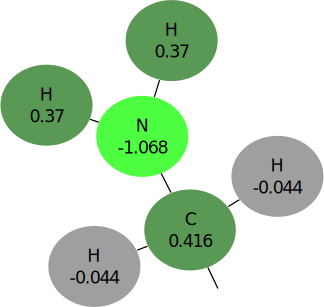
\includegraphics[width=.8\textwidth]{img/match_target.pdf}
\caption{Match target.}
\figlab{match_target}
\end{subfigure}%
\begin{subfigure}[t]{0.5\textwidth}
\centering
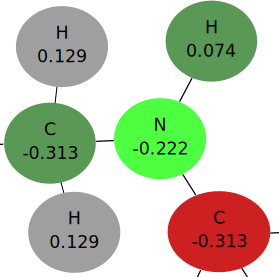
\includegraphics[width=.8\textwidth]{img/match_none.pdf}
\caption{Non-matching fragment.}
\figlab{match_none}
\end{subfigure}%
}\\[1em]
\makebox[\linewidth][c]{%
\begin{subfigure}[t]{0.5\textwidth}
\centering
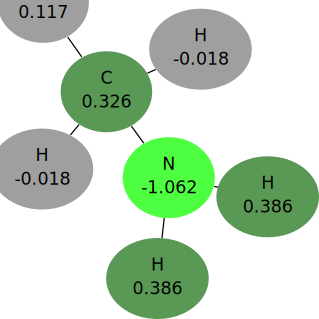
\includegraphics[width=.8\textwidth]{img/match_good.pdf}
\caption{Matching fragment.}
\figlab{match_good}
\end{subfigure}%
\begin{subfigure}[t]{0.5\textwidth}
\centering
\includegraphics[width=.8\textwidth]{img/match_bad.pdf}
\caption{Matching fragment.}
\figlab{match_bad}
\end{subfigure}%
}
\caption{Basic fragment matching.}
\figlab{matching}
\end{figure}

A possible alternative method of finding atom charges is to exploit the similarity of molecules. The partial charges of an unparameterised molecule can be retrieved from similar fragments of other molecules for which the charges \emph{are} known. In \figref{matching}, the basics of fragment matching are shown. In this case, we are looking for an $N$ atom, with two connected $H$ atoms and a connected $C$ (see \figref{match_target}). As can clearly be seen, \figref{match_none} is not a match, as there are two $C$s connected to the $N$ atom there, and only one $H$. \Figref{match_good, match_bad} show two different fragments that \emph{do} match the target fragment. The $N$ atom is indeed connected to a $C$ and two $H$ atoms in both molecules. We will discuss fragment matching in more detail in \secref{impl_omfraf}.

As can be seen clearly for the $C$ atom in \figref{match_good, match_bad}, charges in similar fragments can still differ. This is due to the fact that atom charges are not only influenced by their direct neighbours, but also by the structure of the rest of the molecule. Due to this, it is not yet possible to fully automate the fragment-based molecule parameterisation process, as there are currently no known rules as to which aspects of the structure influence the charge in which way.

Instead of automating the process, a tool needs to be developed that allows experienced chemists to manually perform the atom charge assignment using fragments of other molecules. This tool should provide them with a list of matching fragments, and leave it to them to find the fragments that properly match with the molecule. In order to do this, users should be able to check all aspects of the found fragments, as these determine whether a fragment is a good match or not. Additionally, they need to be able to easily compare fragments, both with each other and with the target molecule.



\section[Challenges]{Interaction design challenges}
\seclab{id_challenges}
A system for fragment-based molecule parameterisation is not readily available. Therefore, a new system needs to be designed from the ground up. This allows for creating something completely new, but also creates the challenge of doing it right without having any clear starting point. In order to be able to validate the system, we implement two different versions of it and compare them.

Both implementations need to meet the same set of requirements. First of all, the system needs to provide its users with a view of the unparameterised molecule, and help them to find the best matching fragments. As the selected fragments may not always be perfect, it should also be possible for the users to manually adjust the charges for each atom, if they feel that this is needed.

In order to make sure users find the best available matching fragment, they should be encouraged to check as many fragments as possible. However, when many fragments are found, users should not have to compare all of them, as this might cost them way too much time. Therefore, the best matches should be easily recognisable, which requires the found fragments to be presented in a clear and intuitive way.

Another important requirement for the system is that is needs to support parameterisation of both small molecules, consisting of just a few atoms, and large molecules, being over a hundred atoms in size. This means that visualisation of the molecules should be given some thought, in order to make sure both large and small atoms are displayed correctly. It is particularly challenging to find a way to properly visualise large molecules on a screen with a limited size, so an approach is needed that allows for this.

Overall, the most important requirement for the system is to make it work intuitively and to implement it such that it makes chemists' work easier. Parameterising a large molecule should therefore not take hours to complete. Even if that would still be faster than calculating the charges, one can at least do something else while the computations are running. This, of course, is not possible while one has to focus on a manual parameterisation process.

\chapter{Related work}
\chlab{relwork}

Quite a lot of literature is available that relates to interaction design for systems like the tool for fragment-based molecule parameterisation that is discussed in this thesis. The literature has been divided into four different categories, each of which discusses a number of papers. Additionally, supporting literature for the work discussed here can be found in \appref{relwork_extra}.


\section{Molecule parameterisation}
\seclab{simulations}
For running molecular simulations, a force-field model describing a molecule's interatomic interactions is required~\cite{canzar2012charge}. In the simulations, the force field requires a specific topology, which includes the molecule's atom types, bonds, bond angles and atomic charges. Using this information, a molecule can be divided into a set of non-overlapping charge groups: sets of \emph{connected} atoms each of which' charge is ideally equal to the molecule's total charge. The work of Canzar, El-Kebir, et al. shows the need for finding the atomic partial charges of a molecule, as these are required for finding the charge groups, which in turn are essential for running molecule simulations.

Malde et al. present the Automated Force Field Topology Builder~(ATB)~\cite{malde2011automated}. The ATB is a web service that can provide topologies that can be used in molecular simulations. It can both act as a repository for molecules that have already been parameterised, and is able to parameterise molecules itself. This automatic parameterisation involves quantum mechanical calculations, which are very complex and computationally intensive. As it is believed that there is no way to speed up these calculations, a new approach is needed, using which atomic charges \emph{can} be found quickly. The topologies that are currently present in the ATB can be used to verify the new approach, by comparing the charges found with the new approach to the charges that are present in the ATB topologies.


\section{Interaction design}
\seclab{design}
% Besides trying to optimise the preparation steps for molecule simulations, the main challenge of this thesis project is to come up with a good interaction design for a tool that does that. In the interaction design area, Donald Norman is a respected and often cited author. He feels that technology can only live up to its full potential by, first of all, supporting human tasks, while making the supporting technology as transparent as possible~\cite{norman2002design}. This can be achieved by making the tools easy to use, easy to learn and easy to understand. Designing for this purpose is called user-centred design.

One of the most important aspects of design is visibility~\cite{norman2002design}. Every interface should have visible features that can send the right messages to the user. It is very important that user actions do not have coincidental consequences. Otherwise, the user can develop wrong expectations of his actions, which may later result in problems while using the tool. What is also important, is that if a user \emph{does} make a mistake, he should be able to undo this. When this is \emph{not} possible, he may get easily frustrated and will stop using the tool. Additionally, the interface should not get in the way of the task that needs to be performed, leading to the user spending his time `using the interface', but should rather help him executing his tasks~\cite{norman1990interfaces}. Finally, the user should not get lost in an giant list of features. As many of these features will often rarely be used, tools with less features, or where the advanced features are presented in a non-obtrusive way, are often the better ones.

When doing interaction design, one has to keep in mind that the appearance of a tool can have great impact on how well the user of that tool can carry out the tasks the tool is intended for~\cite{norman2002emotion}. Tools that are unattractive tend to focus the mind, which leads to better concentration. For tasks where something needs to be done quickly, this is good, but in cases where creative thinking is required, this will not provide a satisfying result. In that case, the thought processes should be broadened by having something that looks really good, thereby slightly distracting the user and allowing him to use creative thinking.

Not only the appearance of software tools is important, also the form in which the information it comprises is presented can make a big difference. For certain types of data, it is highly beneficial to be represented in a visual form. This allows the viewers to perceive patterns and relationships that might be missed in tables and numbers~\cite{gallopoulos1994computer}. Providing users with the ability to modify view parameters at runtime can increase the benefits even further, as they then have the freedom to explore every aspect of the data. However, as discussed before, these options can cause the application user to get lost in the list of options, no longer being able to execute the task he wants to perform. Therefore, the options should be located in some initially closed menu.

% Despite the fact that the importance of design has been long known, many software products are still poorly designed. In an attempt to overcome this, an approach called human-centred design (HCD) has been developed~\cite{norman2005human}. However, even though the needs of the user play a central role here, many companies following the HCD principles still develop complex and confusing products. The systems are often superb at the level of the static, individual display, but fail to support the sequential requirements of the underlying tasks and activities. Therefore, a new approach is needed that does not put the user in a central role, but rather does so with the activity that needs to be performed. In this Activity-Centred Design~(ACD) method, it is sometimes necessary to ignore a user's requests, as they might compromise the task that has to be carried out.

% This, however, does not mean that the application user's needs should be completely ignored. On the contrary, it is really important that the user's characteristics are understood and used in the design of an application~\cite{badre2002shaping}. Also, a good analysis of the context is needed to make the right design decisions. If one ignores the user characteristics and context of an application, the application is  likely to fail, as the context in which the application is developed will almost always differ from the context in which it will be used.

% \subsection{Learning}
% \seclab{id_learning}
% In order to determine what makes a good interaction design, it needs to be known how people learn new things and how our problem solving system works. There are two main learning mechanisms: schema acquisition, where knowledge of subject matter is organized in schemas that determine how new information is dealt with, and the transfer of learned procedures from controlled to automatic processing~\cite{sweller1994cognitive}. Well learned material can be processed automatically, without much effort, while new or less familiar information needs to be processed in a controlled fashion. This means that, when learning something new, one can only use that knowledge by devoting considerable cognitive effort to it. After getting more familiar with the task, the skill may become automatic. Only then can intellectual performance attain its full potential.

% In order to facilitate learning, the process of schema acquisition needs to be triggered and supported. Trying to teach by only providing examples will eventually even have the opposite effect. The learner will then be able to execute the task under the conditions that are equal to those in which he learned the skills, but will fail to do so in other cases. In order to overcome this, teaching should be done using goal-free problems. These problems focus on achieving various problem states and the steps on how to get there, which is exactly how schema acquisition works.

% How easy it is to learn something new is highly dependent on the level of interactivity between the different elements of a task. If there is no interaction between two elements, they can be learned in isolation, requiring less cognitive load than when they have to be learned simultaneously. However, making something easy to learn is not as simple as reducing the element interactivity, as it is dependent on the knowledge of the individual what constitutes an element. For the more experienced, an element may be a whole chunk of the information, while for the rest it may just be an atomic part of the information. Luckily, it is only hard to learn something new when both the intrinsic and extraneous cognitive loads are high. When there is only one high load, the lack of the other compensates for this.

% There are two types of problems: well-structured problems and ill-structured problems. In a well-structured problem, the initial state is well-defined, the goal state is known, and there is a limited set of logical operations to solve the problem~\cite{jonassen2000toward}. If either of these is missing, the problem is classified as being ill-structured. Ill-structured problems are generally more complex than well-structured problems, and are therefore often harder to solve.

% Besides the complexity, there are also many individual differences that determine how easy it is to solve a problem. First of all, when a person is familiar with the domain of a problem, it will be easier to solve for him than it will be for someone with less domain knowledge. Second, more analytical thinkers are often good problem solvers. They must believe that there will be a way to solve the problem, especially when the problem is ill-structured, as they might otherwise just give up before finding a solution. It also helps when someone has a certain affection with the problem. He will then be more likely to try and find the solution. If, however, one has certain beliefs or attitudes about a problem and its solution, he might be a less effective problem solver due to over-relying on that solution. Finally, every problem is different and requires different skills to solve. It can be easier to solve the problem for someone who is familiar with the problem type, but one may never forget that every problem requires a different way of learning.

\subsection[Principles]{Interaction design principles}
\seclab{id_principles}
Following the previously discussed and other research, a number of principles of interaction design can be identified. %However, different authors have different opinions on what those principles are.
Norman and Nielsen identify the following principles of interaction design that are completely independent of technology~\cite{norman2010gestural}:
\begin{itemize}[noitemsep,topsep=0pt,parsep=0pt,partopsep=0pt]
\item Visibility (also called perceived affordances or signifiers);
\item Feedback;
\item Consistency (also known as standards);
\item Non-destructive operations (hence the importance of undo);
\item Discoverability: all operations can be discovered by systematic exploration of menus;
\item Scalability: the operation should work on all screen sizes, small and large;
\item Reliability: operations should work and events should not happen randomly.
\end{itemize}
% Thimbleby, on the other hand, \emph{does} relate his principles to technology~\cite{thimbleby2007press}:
% \begin{itemize}[noitemsep,topsep=0pt,parsep=0pt,partopsep=0pt]
% \item Use good algorithms for better user interfaces: interactive devices are designed to solve problems in a structured way, which is exactly what a good algorithm does;
% \item Use simple, explicit interaction frameworks: those provide clear interaction structures, which allow for reliable feature integration, checking, analysis, fault identification, and error fixing;
% \item Interrelate all interaction programming: all aspects of the design should come out of the same specification;
% \item Define properties and analyse designs for them.
% \end{itemize}
% A more extensive list is provided by Blair-Early and Zender~\cite{blair2008user}:
% \begin{itemize}[noitemsep,topsep=0pt,parsep=0pt,partopsep=0pt]
% \item Obvious start: design an obvious starting point;
% \item Clear reverse: design an obvious exit or stop;
% \item Consistent logic: design an internally consistent logic for content, actions, and effects (the most important consistency is that with user expectations);
% \item Observe conventions: identify and consider the impact of familiar interface conventions;
% \item Feedback: design tangible responses to apt user actions;
% \item Landmarks: design landmarks as a reference for context;
% \item Proximity: design interface elements in consistent proximity to their content objects and to each other;
% \item Adaptation: design an interface that adapts or is adapted to use;
% \item Help: as necessary, provide a readily accessible overall mechanism for assistance;
% \item Interface is content: design interface elements that minimise interface and maximise content.
% \end{itemize}

% The above lists of principles are all quite different, but all consider automation of certain processes. The next section will discuss this in more detail.

\subsection{Automation}
\seclab{id_automation}
Software and artificial intelligence developments allow for increasing possibilities in automating processes. The amount of interaction between humans and computers can be reduced, allowing humans to concentrate on other tasks~\cite{payne2000varying}. However, it depends on the situation when automation should be applied and to what extent. Automation reduces people's situational awareness, which may be undesirable in some environments. Furthermore, it may leave users feeling out of control or can lead to deskilling if decisions are being made autonomously, rather than having a system that is only giving advise.

In order to determine what level of interaction is suitable for a task, multiple interaction methods need to be designed. These often include a `naive' version that only does validation of user input, a `cooperative' version in which the user is given advise on what to do, and a mostly automatic `autonomous' version that only requires some initial parameterisation~\cite{payne2000varying,horvitz1999principles}. In a case study on route planning agents it was found that, for that purpose, the cooperative version delivered the best results~\cite{payne2000varying}. The users of the autonomous version complained they lacked the possibility to fully control the system, while those who used the naive version complained the route planning process was tedious. However, this does not mean that the cooperative version is the silver bullet for man-machine interaction. In some cases, having full control might be necessary, or in other cases, where time consumption is really important, an autonomous version might be preferred.

Cooperative or mixed-initiative user interfaces have been studied in more detail by Horvitz~\cite{horvitz1999principles}. He has found that, in order for automation to work, automated activity should not occur before a user is ready for it. Delays in automation, on the other hand, can diminish its value, so it needs to be carefully timed. Among the most important factors for successful semi-automatic applications are: considering the computer's uncertainty about a user's goals, inferring the ideal action in light of costs, benefits and uncertainties, minimizing the cost of poor guesses, and providing mechanisms for efficient agent-user collaboration to refine results.

An example of a system that has implemented this cooperative interaction design is \verb|SALT|~\cite{marcus1987taking}, a tool for generating expert systems that are to be used in problem solving. Using \verb|SALT|, one will incrementally construct a design by either accepting or rejecting proposed design parameters, one parameter at a time. Constraints will constantly be checked, and, once a constraint violation is detected, the system will try to automatically remedy this. As it is extremely difficult to develop a system that has to perform a task for which expert knowledge is required, \verb|SALT| offers ways to backtrack the assigned parameters. It automatically detects parameters that might need to be modified, but require additional domain knowledge to be fixed properly.

At every step in \verb|SALT|'s incremental parameter assignment, the proposed values are provided in such order that the ones having the least negative effect come first. However, as this does not consider future assignments of other parameters, this means that the assignment may not always converge to a proper solution. This is where the previously discussed backtracking will be useful to see where the `wrong' decision has been made. In two field studies, \verb|SALT| has been proven a good and useful tool for problem solving. However, it has also been found that the required degree of interaction can vary among different systems. Therefore, one should always study the context of a system before deciding on the level of interaction that system will have.

% Automation is often said to be causing problems and to increase the chances for human error when failures occur. Norman proposes in~\cite{norman1990problem} that this is not the cause of automation itself, but rather of the automated systems' lack of appropriate feedback when humans need to take over control. In regular conditions and some predefined exceptional situations, automated systems are perfectly able to operate. It is in those other abnormal situations that automated systems often fail; both in executing their task and alerting the user that something unusual is happening. In order to overcome this, automated systems should be designed while keeping in mind that errors will occur. An appropriate feedback system needs to be present that allows for human intervention when needed.

% An often used, but wrong way of alerting a system's user that something is wrong, is the use of alarms for every component of the system~\cite{norman1990problem}. In exceptional situations, multiple components will often fail at the same time. When all of these would sound an alarm, the user could get confused and will not know what component requires immediate attention and what can wait. Rather than this, systems should continually inform the user about their state, such that he can detect exceptional situations and act upon them. Still, this information should be non-intrusive and presented in a natural way, such that man and machine can jointly solve the problem at hand.

\subsection{Abstraction}
\seclab{id_abstraction}
In order to be able to properly discuss an interaction design, this design needs to be represented at an abstract level. In~\cite{brehmer2013multi}, Brehmer and Munzner describe a multilevel typology for visualisation tasks. This typology consists of the answers to three questions: \verb|why| the task is performed, \verb|how| the task is performed and \verb|what| it pertains to. A list of predefined nodes is provided with which those questions must be answered. By comparing multiple of these typologies, one is able to reason about the differences between two systems on an abstract level, which can be used to hypothesise what system will work better under which circumstances.


\section{Molecule software}
\seclab{software}
There is a lot of software available for displaying, drawing and editing molecules. These programs form an indispensable part of every molecular processing system~\cite{ertl2010molecular}. Throughout the years, molecule software has evolved from basic text editors, through clickable image maps, to full-on molecular structure sketching software. In the last few years, a new trend becomes visible. More and more cheminformatics applications are being brought to the web, allowing for many new ways of interaction. Furthermore, these new applications are being open sourced, allowing for new innovative variations or combinations of the old tools.

An example of a previously offline, closed source tool is \verb|JSmol|, originally known as just \verb|Jmol|~\cite{hanson2013jsmol}. This tool has been seamlessly transformed from a \verb|Java| applet to \verb|JavaScript|, without any visible visual difference. Furthermore, performance wise, there is only a minor difference between the two implementations. Another example is \verb|JSME|~\cite{bienfait2013jsme}, a tool that has been cross-compiled from its original \verb|Java| code to \verb|JavaScript| using the \verb|Google Web Toolkit| compiler. The transition to the web has resulted in the addition of several features, suggested by users from the new, bigger audience. What can be concluded from these two cases is that bringing molecule software to the web opens up a whole world of new possibilities, without having to give up on performance.

With the ongoing migration of molecule software to the web, new devices, such as smartphones and tablets, will be able to run the tools. As these devices promote different ways of user interaction and often have smaller screens, designs of the molecule software need to be reconsidered. \verb|TB Mobile| is a mobile app for identification of potential anti-tuberculosis molecules~\cite{ekins2013tb}. The app is structured in such way that there is always a small control bar at the top, and a large area for showing the content. Interaction with the app is handled by a small number of large buttons, allowing for easy touch controls. In order to work for different screen sizes, everything in the content area is scalable, and, in case not everything fits on the screen, scrollable. Usage of the app in practice has shown that it helps to improve the work flow of tuberculosis researchers, by lowering the barriers for accessing the information it provides.

The issue of showing a lot of data on a limited-size screen is also addressed by Ertl and Rohde~\cite{ertl2012molecule}. They took the concept of a word cloud, and transformed that to the so called Molecule Cloud. Here the highest scored molecules are the biggest and the lowest are the smallest, just like the highest and lowest scored words in a word cloud. None of the molecules overlap, and the sizes are divided such that the whole available screen space is filled. User studies have shown that these molecule clouds provide an easy way of finding the most relevant molecules. However, when many molecules need to be displayed in a small area, this means that either all molecules will be very small, or the lowest scored molecules need to be left out completely. Depending on the situation, this may not be desirable.

\subsection{Molecule visualisation}
\seclab{ms_visualisation}
An important component of molecule software is the visualisation of the molecules. Molecules can be represented in a textual format, but it is often beneficial to use a visual representation, as this can help to illustrate various chemistry phenomena, such as the atomic structure. A study on Finnish upper secondary schools has shown that molecular modelling can truly be valuable~\cite{aksela2008computer}. The fact that students could interact with the models made it easier for them to quickly understand new chemical phenomena, and increased their interest in the subject.

% Molecule visualisation is generally done using either two-dimensional schematic views, or three-dimensional structure models. Which of these forms is best depends on the application for which the visualisation needs to be used. In cases where correct perception of the molecule structure including bond angles, bond lengths, and atom sizes is needed, 3D representations need to be used. A study on Slovenian primary and secondary schools has shown that, for understanding chemical concepts, 3D models are highly beneficial if they can be interacted with~\cite{ferk2003students}. However, as they convey more information than the 2D representations, it does take more time for the students to understand the 3D models. Furthermore, as the structures often have to be converted to a 2D form which the students can draw in their notebooks, transition rules need to be taught, which increases the steepness of the learning curve even further.

In cases where detailed molecule information needs to be described in an abstract way, two-dimensional schematic views, as opposed to three-dimensional structure models, are usually the most useful~\cite{zhou2009molecular}. In a 2D view, one can easily view every atom of a molecule, without having to rotate it. Furthermore, it can easily show which atoms are connected and what type of bond connects them. This creates a good overview of the molecule, and allows for easy comparison of two molecules.

For digitally visualising a molecule, a textual representation of it is needed that can be interpreted by a computer and transformed to a form that includes positional data. There are many different textual molecule formats, including \verb|SMILES|~\cite{daylight1992daylight}, \verb|InChI|~\cite{heller2013inchi}, \verb|Mol2|~\cite{tripos2005tripos}, and \verb|PDB|~\cite{bernstein1977protein}. Each of these formats serves its own purpose. \verb|SMILES| is mainly concerned with expressing atom types and bonds, \verb|InChI| adds charge information, \verb|Mol2| contains information about 2D or 3D atom positions, and \verb|PDB| files contain a lot of additional information about the proteins they describe.

% When a molecule in a textual format that lacks positional information needs to be visualised, its atoms' positions need to be calculated. Starting from the 1970s, algorithms for schematically displaying molecules in 2D have been developed. Dittmar, Mockus and Couvreur created one of the first programs that converted a connection table to a structural molecule diagram~\cite{dittmar1977algorithmic}. Back in the day, computing power was limited, which meant that advanced operations to eliminate overlap in the visualisation needed to be limited. Nevertheless, computing the diagrams still took over three minutes for an average sized molecule. Since then, advances in computer hardware and algorithm improvements have made it possible to speed up the structural diagram generation to times of under a second~\cite{fricker2004automated}. The improvements of computer hardware also allowed for better overlap prevention in the diagrams, leading to much cleaner visualisations~\cite{clark2006structure}. However, overlap is still not completely eliminated, so there is a need for further improvements in these algorithms.

In order to find the positional data of a molecule, it is possible to implement a position calculation algorithm, or use an existing system for this. Alternatively, as data formats including the positional data also exist, it is also possible to obtain this data by converting the input file to a format that does include it. Several systems exist that do this, including \verb|ChemAxon Molconvert|~\cite{chemaxon2014molecule} and \verb|Open Babel|~\cite{oboyle2011open}. \verb|Molconvert| is a closed-source, commercial program that is part of the \verb|ChemAxon Marvin| package. It allows for conversion of most accepted formats, but can only be used in production after buying a license. \verb|Open Babel| on the other hand is an open-source, free to use chemical toolbox. It supports even more formats than \verb|Molconvert|, but its atom position calculations are slightly less accurate.

As a molecule can essentially be seen as a graph of bounded degree with labelled nodes and edges, certain aspects of graph visualisation can be used when drawing molecules~\cite{boissonnat2001structure}. For very large molecules, graph reduction algorithms may provide a way to fit the whole molecule on a limited size screen~\cite{batagelj2004pajek}. Nodes of that reduced molecule can then be expanded to reveal true parts of the molecule, and cut-outs of the whole molecule can be shown to see only relevant parts of the molecule. In some cases, however, it may be necessary for the application user to see every atom of the molecule at all times. It is therefore application dependent if, and to what extent graph visualisation aspects can be applied to molecule visualisation.

\subsection{General requirements}
\seclab{ms_requirements}
In the earlier discussed study on the use of molecule visualisation software in chemistry education in Finnish secondary education (see \secref{ms_visualisation}), and another study on the user of computer programs in biology~\cite{taylor2013interface}, several requirements for molecule modelling programs have been identified. Molecule modelling software should be easy to use, visually appealing, able to save information, and moderately priced~\cite{aksela2008computer}. Furthermore, it should allow its users to rotate and scale molecules, and have logical ways of interaction. Additionally, it is highly beneficial to have different visual representations of the molecule, or to at least be able to modify the visualisation parameters at runtime. This allows the application user to fully tailor the visualisation to his needs. Finally, a clear and extensive manual is needed that not only describes the basic features of the system, but also the more advanced aspects is great detail.


\section{User studies}
\seclab{user_studies}
In Software Engineering, an often used method to evaluate a project is performing a user study. One type of user studies is the experiment, in which two (or more) different configurations of the examined tool are compared~\cite{wohlin2003empirical}. It is important to define exactly what one wants to validate, which should preferably be something that can easily be observed (e.g. `time required' or `number of clicks', but not `comprehensibility')~\cite{stein2009assessing}. Furthermore, it is important that all different configurations are semantically equivalent (i.e. doing the same thing), have an equal degree of compression (i.e. contain the same information) and are formatted into their cleanest and clearest extent.

% Before starting an experiment, it is very important to make sure the subjects are committed to the tasks they need to perform. Otherwise, the experiment will not properly reflect the production environment. Furthermore, the experiment should be well-prepared, as start-up problems might negatively impact the subject's opinion otherwise.

Another type of user studies is the survey. In a survey, it is easy to test a large number of variables, but one should be careful not to test too many, as this will make the analysis infeasible~\cite{wohlin2003empirical}. In order to collect questionnaire information in a structured way, its questions should follow some natural flow that embodies all aspects of a user's experience~\cite{tuch2013analyzing}. This encourages them to report their detailed experiences, as this is less demanding than answering one big open question. Furthermore, it also reduces the chances of subjects failing to report certain things, simply because they forgot about them.

A variety of predefined surveys is available for usability testing, including \verb|SUS|~(System Usability Scale)~\cite{brooke2013sus} and \verb|UMUX|~(Usability Metric for User Experience)~\cite{lewis2013umux}. \verb|SUS| consists of ten items, each of which should be graded on a scale of 1 (strongly disagree) to 5 (strongly agree). From these items, a total score on a scale of 0-100 can be calculated, with the average system scoring 68 points~\cite{sauro2011measuring}. \verb|SUS| has been extensively tested and has shown to be very reliable, both in general and in comparison with other surveys. It has also been found to deliver correct results even when the number of test subjects is small, with a correctness score of over $90\%$ for a group of only 10 people~\cite{tullis2004comparison}.

The \verb|SUS| questionnaire comes in two variants: one with alternating positive and negative statements, and one with only positive ones. The latter of these has been shown to have a higher reliability, presumably due to the effects of the alternating meaning of (dis)agreeing with a statement, which may confuse the user~\cite{lewis2013umux}. This finding has lead to the development of \verb|UMUX-LITE|, a questionnaire consisting of just the positive statements of \verb|UMUX|. \verb|UMUX-LITE| has been shown to yield results of equal reliability as those of the complete \verb|UMUX|, despite the fact that it consists of just two questions. Even though it is less reliable than \verb|SUS|, it is believed that when a system is subjected to both of these surveys, one can get very reliable results on the usability of that system.

% On a final note about surveys, the fact that they are often straightforward makes them perfectly suitable for being held over the internet. It has been shown that the results of online surveys do not significantly differ from their offline counterparts~\cite{komarov2013crowdsourcing}. However, face-to-face surveys are still the only way that allows both the interviewer and the test subject to immediately ask and answer questions~\cite{wohlin2003empirical}. Nevertheless, the effects of this are considered minimal and can often be mitigated by asking the test subject if he has any questions in the questionnaire.

% Before analysing the data obtained by a user study, it is important to validate it~\cite{wohlin2003empirical}. All the obtained results should be complete and correctly documented. Furthermore, extreme outliers should be identified dealt with. What should happen exactly depends on the situation, but in most cases it is best to leave out the extreme results~\cite{komarov2013crowdsourcing}. Finally, it is very important to provide a grade of validity along with the conclusions of the user studies. This grade depends on, for instance, the number of test subjects, their representativeness or the distribution of the results.

\chapter{Research approach}
\chlab{approach}

In this project, as discussed before, a tool for fragment-based molecule parameterisation will be developed and implemented, in order to answer the research questions that were discussed in \chref{introduction}. In this chapter, the taken approach will be discussed. 

From the fact that the idea of fragment-based molecule parameterisation is a new concept, it comes as no surprise that there are no existing tools for this. Furthermore, no tools exist that allow for easy comparison of molecules - or fragments of them - either. This means that there is no baseline to which the developed tool can be compared. In order to still be able to say something about the quality of the tool, two different implementations of it will have to be made~(see \secref{ra_versions}).

In order to evaluate the two implementations, both of them will be subjected to a user study~(see \secref{ra_studies}). This will help to determine if the system works properly and whether it is really fit for the molecule parameterisation task. The project's research questions will be able to be answered, and the hypotheses that will be discussed in \secref{ra_hypotheses}, evaluated.


\section{Two versions}
\seclab{ra_versions}
There are a few axes along which the differences between the two implementations can be made. One could, for instance, compare two tools with varying visualisation methods. Visualising molecules, however, is a well-exhausted field of research, leaving very little room for new ideas.

Another possible variable in the tool is the way its users will interact with it and especially its degree of automation. Varying this degree has been the subject of several studies~(e.g.~\cite{payne2000varying, horvitz1999principles, marcus1987taking, norman1990problem}, see also \secref{id_automation}), all of which concluded the degree to which automation can be applied is highly dependent on the context of the system and sometimes even to the situation in which the system is used.

As discussed in \secref{id_automation}, usually three levels of automation are implemented, creating a naive, cooperative and autonomous version of the system~\cite{payne2000varying}. As it is considered hard to parameterise a molecule based on fragments of other molecules, and little is known on what is the best way of doing this, an autonomous version of a tool that does this cannot yet be developed. The other two versions, however, seem to be perfectly implementable and both can be considered useful.

It has therefore been decided to implement a naive version of the system that has barely any automation at all, and a cooperative version that will continuously make suggestions to the user. They have been called the consuming and producing version respectively~(see \secref{id_versions}). In \chref{design}, the interaction designs for these two versions are discussed in detail, and their implementations are covered in \chref{implementation}.



\section{User studies}
\seclab{ra_studies}
As mentioned before, both versions of the developed system will be subjected to a number of user studies. Unfortunately, not just anyone can be asked to partake in this experiment, as it is a system that is aimed to be used by experienced chemists who understand the details about molecule parameterisation. Luckily, project supervisors Klau and El-Kebir keep a close connection with a substantial group of chemistry researchers, creating the opportunity of asking them to participate in a user study. They were interested in the concept of fragment-based molecule parameterisation, and willing to test a system that does that.

In the user studies, the participants will be split up in two groups, where each person is randomly assigned to a group and both groups are of equal size. This way, it is made sure that both groups are representative, which is essential for user studies~\cite{wohlin2003empirical}~(see also \secref{user_studies}). The groups will take part in an experiment that compares the two versions of the molecule parameterisation tool. Due to the limited number of test subjects, every participant will be asked to test both the consuming and the producing version of the system. As the effects of the order in which two systems are evaluated are often remarkable, one group will start the evaluation with the consuming version, followed by the producing version, where the other group will do this the other way around.

For both versions of the tool, the experiment participants will be instructed to parameterise a couple of molecules, after which they will be asked to answer a short questionnaire, containing questions about that specific version of the system. When they have tested and answered questions about both versions of the tool, users will be asked to submit one final questionnaire, containing more general questions about having a system for molecule parameterisation, but will also ask for their preferred version.

Due to the large number of tasks the experiment participants have to complete, it has been decided to have them parameterise only two molecules per version of the system, i.e. four molecules in total. With an estimated time requirement of ten minutes per questionnaire, participants will already be spending half an hour on that. As the experiment should not take up more than an hour of the participants' time, this leaves only 30 minutes for the actual molecule parameterisation. When loading times are considered, it has to be concluded that there is only time for four molecules in total, i.e. two per version.

Even though testing more than two molecules per version of the system would be better, it is not necessarily a problem to only test two. Many problems with a system will be found in the first two test runs, after which the number of newly discovered problems decreases rapidly~\cite{krug2006dont, nielsen2000you}. Despite the fact that some problems may be left undiscovered, the most common flaws will usually be spotted in the first few runs.

As many of the available participants are scattered around the world, and in order to save time, it has been decided to conduct the experiment over the internet. The potential application users will be contacted via email, and use their own machines to run the system. Additionally, they will submit the answers to the questionnaires using some online form.

In order to be able to obtain results from the user studies, an extensive logging mechanism will have to be built into the system. This can then be used later to precisely reproduce the user's actions, in order to mediate the loss of information due to the fact that the user studies are performed over the internet, with no human observing the participants. If any odd results are found, this can potentially help to pinpoint what went wrong, and, more importantly, it can be used to obtain all kinds of statistics about the molecule parameterisation system.



\section{Hypotheses}
\seclab{ra_hypotheses}
According to Jonassen's dichotomy of problems~\cite{jonassen2000toward}~(see also \secref{id_learning}), fragment-based molecule parameterisation is an ill-structured problem. This means that the problem is quite complex and is therefore hard to solve. Due to this, users need to be ensured that there is a way to find a solution, or they will simply give up. This should be the case for both versions of the system, but is better facilitated by the consuming version than the producing one. In the consuming version, users are not relying on a system to automatically come up with suggestions, but rather do everything themselves. They will know that, by simply repeating the same process a few times, they will get a result. The fact that they have everything in their own hands will make them feel more comfortable about getting to a good solution.

In the earlier mentioned study of Payne, Sycara, and Lewis~\cite{payne2000varying}, it was found that the cooperative version of the examined system had great theoretical benefits in time consumption and user guidance, where the naive version excelled in user freedom. In the general, straight-forward cases studied there, the cooperative version delivered the best results, but, in more complex situations, it was no match for the naive version. As fragment-based molecule parameterisation is an ill-structured, and therefore complex problem, it is believed that the following hypotheses will hold:
\begin{quote}
The producing version of the molecule parameterisation system will take less time to use than the consuming version.
\end{quote}
\begin{quote}
The consuming version of the molecule parameterisation system will yield better results than the producing version.
\end{quote}

When the participants of that study were asked what they thought about the different versions of the system, they noted that using the consuming version was a tedious process that cost a lot of time. However, in some more complex cases, they found it really important to have full control of the system. As mentioned before, parameterising a molecule based on fragments of other molecules is a complex task in itself. Therefore, as user satisfaction and result correctness are considered the most important in this case, the following hypothesis about the system in general can be formulated:
\begin{quote}
For a tool used for fragment-based molecule parameterisation, it is better for users to have full, manual control, than to automate certain parts.
\end{quote}

On a more general level, both versions of the interaction design rely on the idea that fragment-based molecule parameterisation should be chemically correct. As this has not been proven yet, this research project aims to help in determining if it is possible. Both versions of the system will be designed in such way that the user should be able to quickly parameterise a molecule. Furthermore, as it has been proven that properly matching parts of molecules have the same atomic charges, the second - for both versions of the system essential - hypothesis is as follows:
\begin{quote}
It is possible to parameterise a molecule based on fragments of other molecules; both correctly and in a reasonable amount of time.
\end{quote}

When this hypothesis does not hold, fragment-based molecule parameterisation will show not to be a good concept after all. This will also render the comparison of the two interaction designs invalid, as both are then designed for a faulty task, and have been evaluated using that. Luckily, the chances for this are small, as the similarity has been proven in theory, and the parameterisation times cannot get much worse than those of the quantum-mechanical calculations.

\chapter{Interaction design}
\chlab{design}

Here will be the interaction designs for the tool\ldots

\nlipsum


\section{Platform}
The requirements of the molecule parameterisation tool have been specified in \chref{problems}. It has been decided to implement the tool in \verb|HTML5| and \verb|JavaScript|, which allows for great portability and availability across different operating systems and platforms. It also makes the tool future-proof, by following the current trend of bringing everything to the web~\cite{ertl2010molecular}, examples of which are \verb|JSMol|~\cite{hanson2013jsmol} and \verb|JSME|~\cite{bienfait2013jsme}~(see also \secref{software}).

Not surprisingly, there are no existing tools for fragment-based molecule parameterisation, as this is a new concept. Furthermore, no tools exist for comparing molecules - or fragments of them - either. What does exist is a wide range of tools and programs for showing and editing molecules. This includes stand-alone molecule drawing software such as \verb|Accelerys Draw|~\cite{accelrys2012accelrys} and \verb|Avogadro|~\cite{hanwell2012avogadro}, two-dimensional web-based molecule editors like \verb|ChemDoodle 2D Sketcher|~\cite{ichemlabs2013chemdoodle}, \verb|Molsoft HTML5 Molecule Editor|~\cite{molsoft2012molsoft} and \verb|Marvin for JavaScript|~\cite{chemxon2013marvin}, and online three-dimensional visualisation tools \verb|JSMol|~\cite{hanson2013jsmol} and \verb|CanvasMol|~\cite{altered2013canvasmol}.

These existing tools will serve as an initial guideline for the tool to be developed, and parts of their implementations may be reused. The rest of the tool, however, will need to be designed and developed from scratch. The design will follow the basic interaction design principles as posed by Norman and others~(see \secref{id_principles}), the knowledge about learing~(see \secref{id_learning}), and keep in mind the insights gained by the developers of other molecule software~(see \secref{software}).


\section{Two versions}
As there is no existing software for fragment-based molecule parameterisation, there is also no baseline to which the developed tool can be compared. In order to still be able to say something about the quality of the tool, two different implementations of it will be made. There are a few axles along which this difference can be made. One could, for instance, compare two tools that have different visualisation methods. Visualising molecules, however, is a well-exhausted field of research, leaving very little room for new ideas. Furthermore, molecules cannot be represented in textual form here, as a visual representation is essential to perceive similarity of fragments~\cite{gallopoulos1994computer}.

Another possible variable in the tool is the way its users will interact with it and especially its degree of automation. Varying this degree has been the subject of several studies~(e.g.~\cite{payne2000varying, horvitz1999principles, marcus1987taking, norman1990problem}, see also \secref{id_automation}), all of which concluded the degree to which automation can be applied is highly dependent on the context of the system and sometimes even to the situation in which the system is used.

When implementing multiple versions of a tool with different levels of interaction, it is often decided to make three versions: a `naive' version without much automation, a `cooperative' version in which the user is given advise, and an `autonomous' version that only requires some parameterisation~(see~\cite{payne2000varying} and \secref{id_automation}). As it is considered hard to parameterise a molecule based on fragments of other molecules and little is known on what is the best way of doing this, an autonomous version of a tool that does this cannot yet be developed. The other two versions, however, seem to be perfectly implementable and both can be considered useful.

\begin{figure}[h!]
\begin{center}
\includegraphics[width=.9\textwidth]{img/complete_id.pdf}
\caption{The two different interaction designs.}
\figlab{id_flows}
\end{center}
\end{figure}

\Figref{id_flows} shows a naive and a cooperative interaction design for the tool that will be developed. Here, the cooperative design has been called the `smart' version to accentuate its differences with the naive version. The following sections will discuss these two interaction designs, the motivation behind them, their workings, and the hypotheses about them.

\subsection{Manual `naive' version}
Just like the naive RPA implementation from~\cite{payne2000varying}, the naive version of the molecule parameterisation tool will only automatically perform user input validation. Besides ordering the matching fragments based on their probability of being a good match, the tool will not give any advise, nor will it automatically infer any values.

\subsubsection{Workings}
The complete set op steps required to fully parameterise a molecule using the naive version of the tool is as follows:
\begin{enumerate}[itemsep=.1em, parsep=.2em, topsep=0em]
\item The user enters a molecule data string (in \verb|SMILES|, \verb|InChI|, or other format). The molecule will be displayed to the user;
\item The user selects a single atom or a group of \emph{connected} atoms;
\item The user clicks the ``Find matches'' button;
\item A list of matching fragments will be shown, ordered such that the highest rated match comes first and the lowest last. The user can browse through them, preview the result of selecting that match and, once he has found what he sees as the best match, select this match. Hereafter, the charges from that match will be assigned to the molecule;
\item
\begin{itemize}[leftmargin=0cm, itemsep=.1em, parsep=.1em]
\item[]{\bf Unparameterised atoms remain}:\\The user selects another atom / list of connected atoms. Back to step 3;
\item[] {\bf Molecule fully parameterised}:\\Continue to step 6;
\end{itemize}
\item When needed, the user can fine-tune the atom charges by selecting an atom and modifying its charge using an input field. In order to assist him in this process, the fragments that were matched to this atom \emph{and} have been selected will be shown.
\end{enumerate}

\noindent
In the matching process, it is possible that an already charged atom is present in another chosen fragment. In the case where these charges differ, the user will be asked to decide what should happen, which can be one of:
\begin{enumerate}[itemsep=.1em, parsep=.2em, topsep=0em]
\item Take the average of the two charges;
\item Keep the current value;
\item Take the new value;
\item Manually enter a value.
\end{enumerate}

\subsubsection{Motivation}
As pointed out earlier, it is important to have a non-automatic baseline to see if automation can work for a certain tool. In this project, the naive version will serve as that baseline. However, it is more than just a baseline; it could also quite possibly work better than any automated version. The same was concluded for the naive RPA in~\cite{payne2000varying}, which was largely outperformed by its more automated siblings, but offered great benefits in situations where full control was required.

In the naive molecule parameterisation tool, the user can manually decide what atoms need to be parameterised and has a clear overview of all matching fragments. Furthermore, he can manually decide what should happen with overlapping fragments and can modify atom charges at any point in the process. This provides the same benefits as the previously discussed naive RPA had.

Another reason why this naive version might work better than an automated one is the fact that this one encourages exploring different options. By providing a list of fragments, rather than proposing a single one, the fragments can easily be compared such that the chances for the best match being selected increase. Furthermore, as the user is free to determine what atoms should be parameterised at which point in time and also to select groups of atoms, he can experiment with the selection size and order, which may lead to better results.


\subsection{Semi-automatic `smart' version}
Inspired on the cooperative RPA from~\cite{payne2000varying}, \verb|LookOut|~\cite{horvitz1999principles}, and \verb|SALT|~\cite{marcus1987taking}, the smart tool for molecule parameterisation continuously makes suggestions to the user. It will do so with possible matching fragments and atoms that might require fine-tuning, and will autonomously solve conflicting atom charges.

\subsubsection{Workings}
Using the semi-automatic version of the tool, the user should follow the following steps in order to fully parameterise a molecule:
\begin{enumerate}[itemsep=.1em, parsep=.2em, topsep=0em]
\item The user enters a molecule data string (in SMILES, InChI, or other format). The molecule will be displayed to the user;
\item The user clicks the ``Find matches'' button. One of the atoms will now be automatically selected and matching fragments will be retrieved;
\item The highest rated match is previewed on the molecule. The user can either accept or reject this proposed match;
\item
\begin{itemize}[leftmargin=0cm, itemsep=.1em, parsep=.1em]
\item[]{\bf Rejected}:\\Remove this match from the list of matching fragments (the user \emph{can} go back to this one if he changes his mind). Back to step 3;
\item[] {\bf Accepted}:\\Assign the charges of the fragment to the molecule. Continue to step 5;
\end{itemize}
\item
\begin{itemize}[leftmargin=0cm, itemsep=.1em, parsep=.1em]
\item[]{\bf Unparameterised atoms remain}:\\Another unparameterised atom is automatically selected and similar fragments are retrieved. Back to step 3;
\item[] {\bf Molecule fully parameterised}:\\Continue to step 6;
\end{itemize}
\item The user can now fine-tune the charges by selecting an atom and modifying the charge using some input field, if he wants to do so. In order to assist him in this process, suggestions will be given on what atoms to fine-tune and to what value they should be adjusted.
\end{enumerate}

\noindent
In the matching process, it is possible that an already charged atom is present in another chosen fragment. When these charges differ, the atom's charge will be automatically calculated from the two charges. Experimentation has yet to show the best way to do this, but, presumably, taking the average of the two will be a good solution.

\subsubsection{Motivation}
One of the most important reasons for developing a tool for fragment-based molecule parameterisation is to speed up the current process that uses quantum mechanical calculations. Having some automation in this tool can help increasing this benefits even further. By suggesting molecule fragments, parameterising a molecule can potentially be done a lot faster than when the user has to manually go through a list of fragments.

By automating certain parts of the parameterisation process, the tool should also be easier to use. One basically only needs to say `yes' or `no' a few times and will therefore be easy to learn. This increases the potential for new people to start using the tool, thereby enhancing its value. Furthermore, it makes sure users do not get lost in a long list of features. Otherwise, users might make the wrong decisions or even stop parameterising completely~\cite{norman2002design}~(see also \secref{design}).

In order to mediate the often occurring problems with automation, the fine-tuning step at the end has been added, based on studies by Norman~\cite{norman1990problem} and Horvitz~\cite{horvitz1999principles}. As there will always be errors in the automatic charge corrections, this provides the user with a way to identify and improve incorrectly assigned atom charges. The warnings that some atoms may be charged incorrectly will be non-intrusive, and the user will be able to see how every charge came to be in order to determine how to improve it.


\section{Interaction topology}
In order to be able to discuss visual interfaces at an abstract level, Brehmer and Munzner have developed a multi-level typology for abstract visualisation tasks~\cite{brehmer2013multi}~(see also \secref{id_abstraction}). The Brehmer-Munzner typology\footnote{It is not officially named, but will be referred to as the `Brehmer-Munzner typology' in the remainder of this document.} for the two implementations of the molecule parameterisation tool is shown in \figref{id_typologies}.

\begin{sidewaysfigure}[p]
\begin{center}
\includegraphics[width=\textwidth]{img/complete_typology.pdf}
\caption{Brehmer-Munzner Typologies of the two different interaction designs.}
\figlab{id_typologies}
\end{center}
\end{sidewaysfigure}

These typologies clearly outline the differences between the two implementations. While the naive version is mainly concerned with presenting things to the user and user exploration, in the smart version, the user is mainly discovering (verifying) the system's proposals and browsing through them. This means that, in the semi-automatic version, the user has easier access to the information, and can therefore make decisions earlier than in the naive version.

What is also clear in the typologies is the difference in the number of different methods that is required to parameterise a molecule in the two versions. In every step of the process, the smart version requires less different methods than the naive one. This does not necessarily mean that the smart version will take less time to use, as the methods may need to be used more often. What it does mean, however, is that it will be easier to use the smart version, as less different methods need to be used and learned~\cite{sweller1994cognitive}~(see also \secref{id_learning}).

\chapter{Implementation}
\chlab{implementation}

Here will be implementation details about the three systems\ldots

\nlipsum


\section[OFraMP]{The Online tool for Fragment-based Molecule Parameterisation}
\nlipsum

\subsection{Visualisation}
\nlipsum

\subsection{Interaction}
\nlipsum


\section[OAPoC]{The Online tool for Atom Position Calculation}
\nlipsum

\subsection{obabel}
\nlipsum


\section[OMFraF]{The Online tool for Molecule Fragment Finding}
\nlipsum

\subsection{Generation}
\nlipsum

\subsubsection{mop/fragments}
\nlipsum

\subsection{Finding}
\nlipsum

\chapter{Evaluation}
\chlab{evaluation}

Here will be the description of the project evaluation\ldots

\nlipsum


\begin{comment}
To evaluate this project's hypotheses~(see \secref{hypotheses}), both versions of the developed tool will be subjected to a number of user studies. Currently, however, the presumed user base is limited to only a small number of researchers. Luckily, project supervisors Klau and El-Kebir keep a close connection with most of those researchers, who work at VU University Amsterdam. They have shown some interest in the tool and are willing to participate in the user studies. Furthermore, as some of the researchers are also teaching, they can ask some of their students to evaluate the tool as well. It is not possible to ask random students, as they will lack domain knowledge, making their results unreliable~\cite{jonassen2000toward}. The researchers' students are considered to have enough domain knowledge to be able to correctly parameterise a molecule.

In the user studies, the test subjects will be split up in two groups, where each subject is randomly assigned to a group and both groups are of equal size and equal student-scientist ratio. This way, it is made sure that both groups are representative, which is essential for user studies~\cite{wohlin2003empirical}~(see also \secref{user_studies}).

The groups will take part in an experiment that compares the two versions of the molecule parameterisation tool~\cite{wohlin2003empirical}. One group will test the naive version, the other will use the smart one. For both groups, every member will be asked to parameterise a few molecules of increasing size and complexity. The first one will be quite easy to complete, but the last one should be of such complexity that, theoretically, using the tool is beneficial over using conventional quantum mechanical calculations. It is in these last situations that the tool should show its true value.

During the tasks, the time required to complete the parameterisation will be measured. The difference between the time required in the two implementations will help deciding which of the two implementations is better, but, for both tools, completing the parameterisation should definitely not take hours to finish. Furthermore, users should not report they are annoyed by the tool or willing to stop parameterising.

Besides time, the user will also be scored on his performance. In order to do this, the molecules that the user will be asked to parameterise should already have been parameterised using the conventional quantum mechanical calculations. This way, the user's results can be compared to the outcomes of the calculations to establish his score. The smaller the difference between the two, the better the performance of the user will be graded. Of course, there will always be a small difference between the manual and calculated ways, as the manual assignment cannot be as precise as the calculated one is. However, as long as the difference is small, the developed tool can be considered useful to speed up atomic charge assignment.

For the experiment, timing and scoring mechanisms will be built into the tool. The timing mechanism will simply measure the time between the first click on the tool's ``Find matches'' button and the moment where the user saves the final parameterisation. This value will be stored in a database, along with the value obtained by the scoring mechanism. This value, as discussed before, will be calculated from the difference between the assigned charges and the previously calculated ones.

In order to be able to explain the scoring results and to evaluate them in more detail, the proposed fragments and the selected ones will also be stored. This way, it should be possible to pinpoint where a user went wrong, if he did. Furthermore, it can also help to identify outliers. If it is clear that someone was just messing around with the tool and did not care about getting a good result, that user's experiment results can be left out.

After completing their tasks, the users will be asked to answer a number of questions about the tool. These will mainly be about how they like the design and if they can see themselves using it, but will also ask them for suggestions on things that can be improved or added. This way, their experiences can be used to further improve the tool, and to make it a tool they really like using.

The questionnaire that test subjects will be asked to fill in will be based on the \verb|SUS| and \verb|UMUX-LITE| usability metrics~\cite{lewis2013umux}~(see also \secref{user_studies}). It will consist of the, for this tool, relevant questions from those metrics, along with some additional application-specific questions. It will be made sure the questions follow some natural flow, in order to encourage the testers to report their detailed experiences~\cite{tuch2013analyzing}. Furthermore, the questions will be somewhat directive, to reduce the chances of test subjects forgetting to report certain things.

The results of the user studies combined with those obtained with the questionnaire should be able to give an answer on which of the two interaction designs is better. The version that gives good results in a short amount of time and is also positively graded in the questionnaire will be the better one. Furthermore, the timing and scoring results from the experiment alone will be able to answer the question if it is possible to do fragment-based molecule parameterisation at all. At least for one of the two versions both time consumption and parameterisation results should be reasonable.
\end{comment}
\chapter{Results}
\chlab{results}

In the user studies, a lot of different types of data has been created. First, graphical representations of most observations from the user action log can be found in \appref{graphs}. In that same chapter, the outcomes of the \verb|SUS| and \verb|UMUX| questions that were asked in the questionnaire can also be found. \Appref{comments} contains all answers to the open questions, including general comments about the system, the preferred version and suggestions for improvement.

This chapter will contain the important and most interesting results obtained in the user studies. Each result will shortly be discussed, and further analysed in \chref{discussion}.


\section{Action log results}
From the logging system that was built into \oframp{} for the user studies, a wide range of information can be gathered, spanning from the load time and the number of clicks on atom 5 to the selected conflict solutions and resulting parameterisation. This section contains the most interesting results that can be retrieved from the action log.

\subsection{Time required}
First of all, it is interesting to see in what version users spent the most time to fully parameterise the molecules. \Figref{graph_time_1} shows the total time that was required for both the first and second set of molecules, in both the naive and smart version of \oframp. What can be seen here is that, for both the first and second set of molecules, users needed more time to complete the parameterisation using the naive version. Users who started with the naive version used the most time overall, with a median total time of around 300 seconds, after which those same users spent the least time on the smart version, where the median time value is around 100 seconds. At around 200 and 150 seconds, one can find the median times required by the users who did the naive version second and the smart version first respectively.

\begin{figure}[h!]
\center
\includegraphics[width=.6\textwidth]{img/graphs/1a_02.pdf}
\caption{Total parameterisation time for the two versions in the two orders.}
\figlab{graph_time_1}
\end{figure}

The total time used to parameterise the first and second sets of molecules can be used to determine what version of \oframp{} is the most time-consuming. However, as both sets of molecules have slightly varying molecule sizes, it may be more interesting to look at the average time that was required per atom. This can be seen in \figref{graph_time_2}.

\begin{figure}[h!]
\center
\includegraphics[width=.6\textwidth]{img/graphs/1a_03.pdf}
\caption{Average time per atom for the two versions in the two orders.}
\figlab{graph_time_2}
\end{figure}

What is interesting to see here, is the fact that, where in the total parameterisation time, the group that did the smart version second was done the fastest, its members have spent the most time on average per atom. When taking a closer look at \figref{graph_time_3} and \figref{graph_time_4}, which show the average time per atom required for all molecules separately, this difference appears to be caused completely by the excessive amount of time users spent on parameterising molecule 13913 in the smart version, which is the first molecule users got to parameterise after they have completed the naive version. Even more interesting to see is the fact that most users spent more time parameterising this 11-atom molecule than on the larger 77-atom molecule 17738.

\begin{figure}[h!]
\centering
\begin{subfigure}[t]{0.48\textwidth}
\centering
\includegraphics[width=\textwidth]{img/graphs/1c_03.pdf}
\caption{Smaller molecules.}
\figlab{graph_time_3}
\end{subfigure}%
~
\begin{subfigure}[t]{0.48\textwidth}
\centering
\includegraphics[width=\textwidth]{img/graphs/1d_03.pdf}
\caption{Larger molecules.}
\figlab{graph_time_4}
\end{subfigure}
\caption{Average time per atom for all molecules in the two orders.}
\figlab{graph_time_34}
\end{figure}

It is hard to say what exactly is causing this difference. It is possible that, after using the naive version, it is hard to get used to the smart version, which is way more restrictive as to what a user can do. However, this difference is not present when switching from the smart to the naive version. This can either mean that this switch is easier to make, or that there must be a different cause of the large time difference.

Another possible explanation for the large increase in time required for parameterising molecule 13913 is that there may not be really good matching fragments, enforcing the user to browse through many of them before being able to select the best one. This is better facilitated by the naive version of the tool, and can potentially have the extreme effects that are observed here.

Apart from molecule 13913, \figref{graph_time_34} shows that finishing a parameterisation using the naive version of \oframp{} requires more time than using the smart one. It is also clear that the time required is much more constant, and, with an overall average of around 7 seconds per atom, overall still the fastest, compared to 10 seconds for the naive version.


\subsection{Parameterisation rating}
Not only the time required by the parameterisation tool is important to determine which interaction design is the best, the quality of the result is also of great importance. As discussed in \secref{analysis}, there are two ways of calculating this quality rating. First, the total difference between the charge found by the user and the charge present in the ATB can be found, as shown in \figref{graph_rating_1}. As this difference can easily be observed and corrected by the user, it would be expected that it would be relatively close to 0. This, however, turns out not to be the case. Especially in the smart version of \oframp, the charge difference can get quite high, and is greater than the charge difference for the naive version in any case.

\begin{figure}[h!]
\center
\includegraphics[width=.6\textwidth]{img/graphs/1a_00.pdf}
\caption{Total charge difference for the two versions in the two orders.}
\figlab{graph_rating_1}
\end{figure}

What is also interesting to note here is the fact that, for both the naive and the smart versions of \oframp, the total charge difference is higher for the second set of molecules. This may indicate that these molecules are harder to parameterise, or that there are no good matching fragments for those molecules available. However, it may also indicate that users were starting to lose their concentration, or were confused due to the switch from one version to another.

Where the difference in the total molecule charge can mainly be used to assess user performance, the correctness of the parameterisation can better be measured using the per-atom charge differences. \Figref{graph_rating_2} shows these differences for the first and second set of molecules, both for the naive and smart version of \oframp. As can be seen in that graph, charge differences are, again, smaller for the naive version than they are for the smart version.

\begin{figure}[h!]
\center
\includegraphics[width=.6\textwidth]{img/graphs/1a_01.pdf}
\caption{Average charge difference per atom for the two versions in the two orders.}
\figlab{graph_rating_2}
\end{figure}

In contrast to the total charge differences though, the average charge differences for the second set of molecules are smaller than those for the first set. This suggests the opposite of what was concluded from \figref{graph_rating_1}: the second set of molecules may be easier to parameterise, or there may be better matching fragments available. This suggestion is more probable, as for the total charge difference a negative offset between two atom charges can be compensated by a positive offset in two others, which is not the case for the per-atom difference.

As can be seen in \figref{graph_rating_34}, the naive version of \oframp{} scores better for all individual molecules. What can also be seen there is the fact that, even on average, the charge differences are bigger for the larger molecules than for the smaller ones. Unfortunately, there is no obvious explanation for this. Probably, larger fragments are used for the larger molecules. When one of those fragments is wrong, it quickly adds up to the atom charge difference. On the other hand, it is also possible that users felt more comfortable selecting small fragments, which are generally worse matches than the large ones, due to less atoms matching between the two molecules.

\begin{figure}[h!]
\centering
\begin{subfigure}[t]{0.48\textwidth}
\centering
\includegraphics[width=\textwidth]{img/graphs/1c_01.pdf}
\caption{Smaller molecules.}
\figlab{graph_rating_3}
\end{subfigure}%
~
\begin{subfigure}[t]{0.48\textwidth}
\centering
\includegraphics[width=\textwidth]{img/graphs/1d_01.pdf}
\caption{Larger molecules.}
\figlab{graph_rating_4}
\end{subfigure}
\caption{Average charge difference per atom for all molecules in the two orders.}
\figlab{graph_rating_34}
\end{figure}

\subsection{Other results}
Besides the time required to complete the parameterisation and its rating, some other interesting things were observed in the user studies. First of all, there appears to be a great correlation between the version of \oframp{} that is used and the amount of actions a user needs to undo, as can be seen in \figref{graph_undo}. Where in the naive version, users practically do not undo any action, there are extreme cases where a user needed to undo over a hundred times in the smart version. This difference can be explained by the fact that users of the smart version have to undo accidentally rejected fragments, or may use a combination of reject and undo actions to compare various fragments.

\begin{figure}[h!]
\center
\includegraphics[width=.6\textwidth]{img/graphs/1a_10.pdf}
\caption{Number of undo actions for the two versions in the two orders.}
\figlab{graph_undo}
\end{figure}

As can be seen in \figref{graph_clicks}, a few more clicks are required to complete a parameterisation in the smart version of the tool, then there are in the naive version. Nevertheless, the medians are not too far apart, so it is not really possible to draw any conclusions from this. It is interesting to see, however, that even though the smart version of \oframp{} requires less user interaction, is does not require less, and possibly even more clicks to complete a parameterisation.

\begin{figure}[h!]
\center
\includegraphics[width=.6\textwidth]{img/graphs/1a_04.pdf}
\caption{Total number of clicks for the two versions in the two orders.}
\figlab{graph_clicks}
\end{figure}

\Figref{graph_help} shows that not many users had to consult the help pages during the parameterisation process. Furthermore, no users checked the help pages in their second version of the system. This can mean that either they did not know there were different versions of the help pages as well, or they did not need it any more. The fact that most users did not go to the help pages at all suggests that the tool is intuitive to use, and that taking the demo provides enough information to be able to use \oframp.

\begin{figure}[h!]
\center
\includegraphics[width=.6\textwidth]{img/graphs/1b_01.pdf}
\caption{Total number of clicks on the help button for the two versions in the two orders.}
\figlab{graph_help}
\end{figure}

There are also a few things users did not do at all. They were not required or instructed to use every aspect of \oframp, but it was expected that they would at least try some of the more advanced features. First, none of the users used any of the available keyboard shortcuts. Although all actions for which a keyboard shortcut exists can also be completed using a single mouse click, it was expected that some users would find it beneficial to use keyboard shortcuts for some actions, but this turned out not to be the case.

Furthermore, and more surprisingly, none of the users manually edited a single atom charge. Again, they were not specifically instructed to do so, but they were made aware of the possibility of doing this, and instructed to make the parameterisation as good as possible. Possibly, users were unable to locate the position of the charge edit fields, but no comments about that have been made. Probably, they just did not feel the need of it, or thought their parameterisation was perfect the way it was.

\subsection{Correlations}
\nlipsum


% TODO fix axis labels saying 'time per FRAGMENT'
\begin{figure}[h!]
\centering
\begin{subfigure}[t]{0.48\textwidth}
\centering
\includegraphics[width=\textwidth]{img/graphs/3a_00.pdf}
\caption{Average charge difference per atom in relation to the average time used per atom.}
\figlab{graph_correlation_1}
\end{subfigure}%
~
\begin{subfigure}[t]{0.48\textwidth}
\centering
\includegraphics[width=\textwidth]{img/graphs/3a_01.pdf}
\caption{Total charge difference in relation to the average time used per atom.}
\figlab{graph_correlation_2}
\end{subfigure}%
\\
\begin{subfigure}[t]{0.48\textwidth}
\centering
\includegraphics[width=\textwidth]{img/graphs/3a_02.pdf}
\caption{Average charge difference per atom in relation to the number of used fragments per atom.}
\figlab{graph_correlation_3}
\end{subfigure}%
~
\begin{subfigure}[t]{0.48\textwidth}
\centering
\includegraphics[width=\textwidth]{img/graphs/3a_03.pdf}
\caption{Average charge difference per atom in relation to the number of original molecule views per selected fragment.}
\figlab{graph_correlation_4}
\end{subfigure}
\caption{Presumed correlations between user studies outcomes.}
\figlab{graph_correlation}
\end{figure}


\section{Questionnaire outcomes}
\nlipsum

\subsection{\texttt{SUS} / \texttt{UMUX} results}
\nlipsum

\begin{figure}[h!]
\center
\includegraphics[width=.3\textwidth]{img/graphs/4a_10.pdf}
\caption{Average rating for the two versions.}
\figlab{graph_rating_1}
\end{figure}

\begin{figure}[h!]
\center
\includegraphics[width=.6\textwidth]{img/graphs/4b_10.pdf}
\caption{Average rating for the two versions in the two orders.}
\figlab{graph_rating_2}
\end{figure}

\begin{figure}[h!]
\centering
\begin{subfigure}[t]{0.32\textwidth}
\centering
\includegraphics[width=\textwidth]{img/graphs/4a_00.pdf}
\caption{Rating of \texttt{SUS1}.}
\figlab{graph_rating_3}
\end{subfigure}%
~
\begin{subfigure}[t]{0.32\textwidth}
\centering
\includegraphics[width=\textwidth]{img/graphs/4a_01.pdf}
\caption{Rating of \texttt{UMUX1}.}
\figlab{graph_rating_4}
\end{subfigure}%
~
\begin{subfigure}[t]{0.32\textwidth}
\centering
\includegraphics[width=\textwidth]{img/graphs/4a_09.pdf}
\caption{Rating of \texttt{SUS10}.}
\figlab{graph_rating_5}
\end{subfigure}
\caption{Selected ratings for the two versions of \oframp.}
\figlab{graph_rating_345}
\end{figure}


\subsection{Comments}
\nlipsum

\chapter{Discussion}
\chlab{discussion}

From the results obtained in the user studies, it can be decided which version of \oframp{} is the best for the task of fragment-based molecule parameterisation. What version that is will be argued in this chapter, along with a description of how it can be improved in the future. Additionally, some threats to the validity of the experiment outcomes will be discussed.


\section{The best version}
There are several factors that can help to determine which interaction design for \oframp{} is the best. First, the time required to complete a parameterisation an be considered. As discussed in \secref{res_time}, the smart version requires the least time per atom, and will therefore be the fastest to completely parameterise a molecule. With a total median time of under five minutes for parameterising all four molecules in the user study, it can also be considered to be fast in general. Time-wise, the smart version is therefore the best.

Second, one can look at the correctness of the resulting parameterisations of the different versions. The results presented in \secref{res_rating} show that the naive version has the lowest overall charge difference for both the first and second set of molecules. Furthermore, it has a lower average atom charge difference for every parameterised molecule as well, with average differences of $0.054$ for the smaller molecules, and $0.146$ for the bigger ones. This means that, result-wise, the naive version is the best.

The final information that can be gathered from the user action log is the number of actions that needed to be undone, and the total number of clicks that needed to be made to complete the parameterisations. As was described in \secref{res_other}, the naive version required almost no undo commands, while the smart version required the use of many. Furthermore, the total number of clicks was also smaller for the naive version, making this the better version in those two aspects as well.

Besides the action logs, the \verb|SUS| ratings of the two versions of the system can also be used to decide which one is best. As discussed in \secref{res_sus}, the naive version scored higher than or equal to the smart version for all but one statement. Additionally, with a total \verb|SUS| score of $76$, it not only had a higher score than the smart variant, but was also graded above average, or `good'.

Comments the user studies participants made on the smart version were less positive than those made on the naive version. This also showed in their preference verdict, where all participants voted for the naive version, rather than the smart variant~(see \secref{res_preference}). Most of them commented they strongly preferred that version.

Combining all of this data, it is clear that the naive interaction design is the better of the two. It gives better results, and is found to be better fit for molecule parameterisation than the smart design. Even though it takes slightly more time to complete a parameterisation in that version, it still is reasonably fast. However, it may not be considered the perfect interaction design yet. Many suggestions on how it could be improved have been made~(see \secref{res_suggestions}), resulting in some future work which will be discussed later in this chapter.


\section{Threats to validity}
As in every research project, there are always a few threats to the validity of its outcomes. For the conclusions on the best interaction design for \oframp, this is no different. Most important here is the limited number of participants in the user studies. Due to the limited amount of people currently involved in manual molecule parameterisation, and the limited amount of time in which they had to complete the experiment~(one week), only 10 people were able to partake. However, it has been shown that a sample size of only 10 people leads to a correct \verb|SUS| conclusion $80\%$ of the time~\cite{tullis2004comparison}.

This limited amount of experiment participants also lead to the decision that every user would have to test both versions of the system. While this is not a bad thing in general, it would have been preferred to do a double-blind test to make sure users were not primed by the first version they used. It has been attempted to mitigate this risk by dividing the participants over two groups, where both would use the systems in a different order, but this does not rule out any effect it may have had on the results.

The fact that users had to test the two versions of the system unfortunately also doubled the time they needed to complete the experiment. Even though the total time it took to complete all parameterisations was under 10 minutes on average, users also had to complete two different demo modes and fill in three questionnaires. This brings the total time for the average user to around 45 minutes, where in extreme cases users took far over an hour from loading the first version to submitting the final questionnaire. This may potentially have lead to loss of concentration, and might have incited users to take shortcuts in the parameterisation process, although this has not explicitly been observed.

By organising the user studies over the internet, there has been no control of the environment in which the participants performed the experiment. Although the users were instructed to make a large time slot available for it, and asked to try to focus as much as they could, it may be possible that they got interrupted at certain points, or used the system in a busy environment. This, unfortunately, is one of the insuperable side-effects of conducting an on-line user study.

Another possible threat to the validity of the results is the choice of atoms for the user study. For the experiment, four molecules (two small, two large) were randomly selected from the \verb|ATB|. It is unknown whether these were good example molecules or not, as they may have some special properties, or similar molecules may not exist at all.

Additionally, as commented by many users, the fragment finding system is not perfect yet. It does sometimes find matches that do not make a lot of sense from a chemistry perspective, and the rating system needs to be improved such that the best matches will in fact also be the highest rated. Even though the development of the fragment finding system was outside the scope of this project, it can still have had some influence on the outcomes.

In order to find the best interaction design for a fragment-based molecule parameterisation system, two different designs have been implemented and compared. Although there was a strong preference for the naive version, it may be the case that a third, completely different system would be even better. However, even though the users had many suggestions on how the system could be improved further, none of these suggestions was really ground-breaking from the interaction design point of view. This does not rule out the possibility of the existence of an even better version, but does reduce the chances for it.

Finally, an unfortunate implementation/design error in the system that stored the user comments lead to the loss of the comments of two users. Although their \verb|SUS| ratings did not really deviate from the others, it may be the case that they made some different comments, or actually picked the smart version as their preferred one. Sadly, there is no way to recover these comments, but the similarity of the \verb|SUS| results suggests that there was no big difference of these users' opinion.


\section{Future work}
\nlipsum
 % With future work section
\chapter{Conclusion}
\chlab{conclusion}

Here, the project's conclusion will be presented\ldots

\nlipsum


\cleardoublepage
\phantomsection
\addcontentsline{toc}{chapter}{Bibliography}
\bibliographystyle{abbrv-rt}
\bibliography{references}
\chaptermark{Bibliography}

\appendix
\chapter{Additional literature}
\chlab{relwork_extra}

Apart from the literature that has already been discussed in \chref{relwork}, additional literature has been consulted to make sure \oframp{} would be designed and implemented properly. This literature will be discussed in this chapter, and uses the same structure and categorisation that was used for the related work chapter.



\section{Interaction design}
Despite the fact that the importance of design has been long known, many software products are still poorly designed. In an attempt to overcome this, an approach called human-centred design (HCD) has been developed~\cite{norman2005human}. However, even though the needs of the user play a central role here, many companies following the HCD principles still develop complex and confusing products. The systems are often superb at the level of the static, individual display, but fail to support the sequential requirements of the underlying tasks and activities. Therefore, a new approach is needed that does not put the user in a central role, but rather does so with the activity that needs to be performed. In this Activity-Centred Design~(ACD) method, it is sometimes necessary to ignore a user's requests, as they might compromise the task that has to be carried out.

This, however, does not mean that the application user's needs should be completely ignored. On the contrary, it is really important that the user's characteristics are understood and used in the design of an application~\cite{badre2002shaping}. Also, a good analysis of the context is needed to make the right design decisions. If one ignores the user characteristics and context of an application, the application is  likely to fail, as the context in which the application is developed will almost always differ from the context in which it will be used.


\subsection{Learning}
\seclab{id_learning}
In order to determine what makes a good interaction design, it needs to be known how people learn new things and how our problem solving system works. There are two main learning mechanisms: schema acquisition, where knowledge of subject matter is organized in schemas that determine how new information is dealt with, and the transfer of learned procedures from controlled to automatic processing~\cite{sweller1994cognitive}. Well learned material can be processed automatically, without much effort, while new or less familiar information needs to be processed in a controlled fashion. This means that, when learning something new, one can only use that knowledge by devoting considerable cognitive effort to it. After getting more familiar with the task, the skill may become automatic. Only then can intellectual performance attain its full potential.

In order to facilitate learning, the process of schema acquisition needs to be triggered and supported. Trying to teach by only providing examples will eventually even have the opposite effect. The learner will then be able to execute the task under the conditions that are equal to those in which he learned the skills, but will fail to do so in other cases. In order to overcome this, teaching should be done using goal-free problems. These problems focus on achieving various problem states and the steps on how to get there, which is exactly how schema acquisition works.

How easy it is to learn something new is highly dependent on the level of interactivity between the different elements of a task. If there is no interaction between two elements, they can be learned in isolation, requiring less cognitive load than when they have to be learned simultaneously. However, making something easy to learn is not as simple as reducing the element interactivity, as it is dependent on the knowledge of the individual what constitutes an element. For the more experienced, an element may be a whole chunk of the information, while for the rest it may just be an atomic part of the information. Luckily, it is only hard to learn something new when both the intrinsic and extraneous cognitive loads are high. When there is only one high load, the lack of the other compensates for this.

There are two types of problems: well-structured problems and ill-structured problems. In a well-structured problem, the initial state is well-defined, the goal state is known, and there is a limited set of logical operations to solve the problem~\cite{jonassen2000toward}. If either of these is missing, the problem is classified as being ill-structured. Ill-structured problems are generally more complex than well-structured problems, and are therefore often harder to solve.

Besides the complexity, there are also many individual differences that determine how easy it is to solve a problem. First of all, when a person is familiar with the domain of a problem, it will be easier to solve for him than it will be for someone with less domain knowledge. Second, more analytical thinkers are often good problem solvers. They must believe that there will be a way to solve the problem, especially when the problem is ill-structured, as they might otherwise just give up before finding a solution. It also helps when someone has a certain affection with the problem. He will then be more likely to try and find the solution. If, however, one has certain beliefs or attitudes about a problem and its solution, he might be a less effective problem solver due to over-relying on that solution. Finally, every problem is different and requires different skills to solve. It can be easier to solve the problem for someone who is familiar with the problem type, but one may never forget that every problem requires a different way of learning.


\subsection{Interaction design principles}
Different authors have different opinions on what the exact principles of interaction design are. Where the earlier discussed principles of Norman and Nielsen are completely unrelated to technology~\cite{norman2010gestural}, others do the complete opposite. Thimbleby, for example, \emph{does} relate his principles to technology~\cite{thimbleby2007press}:
\begin{itemize}[noitemsep,topsep=0pt,parsep=0pt,partopsep=0pt]
\item Use good algorithms for better user interfaces: interactive devices are designed to solve problems in a structured way, which is exactly what a good algorithm does;
\item Use simple, explicit interaction frameworks: those provide clear interaction structures, which allow for reliable feature integration, checking, analysis, fault identification, and error fixing;
\item Interrelate all interaction programming: all aspects of the design should come out of the same specification;
\item Define properties and analyse designs for them.
\end{itemize}
A more extensive list of principles is provided by Blair-Early and Zender~\cite{blair2008user}:
\begin{itemize}[noitemsep,topsep=0pt,parsep=0pt,partopsep=0pt]
\item Obvious start: design an obvious starting point;
\item Clear reverse: design an obvious exit or stop;
\item Consistent logic: design an internally consistent logic for content, actions, and effects (the most important consistency is that with user expectations);
\item Observe conventions: identify and consider the impact of familiar interface conventions;
\item Feedback: design tangible responses to apt user actions;
\item Landmarks: design landmarks as a reference for context;
\item Proximity: design interface elements in consistent proximity to their content objects and to each other;
\item Adaptation: design an interface that adapts or is adapted to use;
\item Help: as necessary, provide a readily accessible overall mechanism for assistance;
\item Interface is content: design interface elements that minimise interface and maximise content.
\end{itemize}


\subsection{Automation}
Automation is often said to be causing problems and to increase the chances for human error when failures occur. Norman proposes in~\cite{norman1990problem} that this is not the cause of automation itself, but rather of the automated systems' lack of appropriate feedback when humans need to take over control. In regular conditions and some predefined exceptional situations, automated systems are perfectly able to operate. It is in those other abnormal situations that automated systems often fail; both in executing their task and alerting the user that something unusual is happening. In order to overcome this, automated systems should be designed while keeping in mind that errors will occur. An appropriate feedback system needs to be present that allows for human intervention when needed.

An often used, but wrong way of alerting a system's user that something is wrong, is the use of alarms for every component of the system~\cite{norman1990problem}. In exceptional situations, multiple components will often fail at the same time. When all of these would sound an alarm, the user could get confused and will not know what component requires immediate attention and what can wait. Rather than this, systems should continually inform the user about their state, such that he can detect exceptional situations and act upon them. Still, this information should be non-intrusive and presented in a natural way, such that man and machine can jointly solve the problem at hand.



\section{Molecule software}


\subsection{Molecule visualisation}
Molecule visualisation is generally done using either two-dimensional schematic views, or three-dimensional structure models. Which of these forms is best depends on the application for which the visualisation needs to be used. In cases where correct perception of the molecule structure including bond angles, bond lengths, and atom sizes is needed, 3D representations need to be used. A study on Slovenian primary and secondary schools has shown that, for understanding chemical concepts, 3D models are highly beneficial if they can be interacted with~\cite{ferk2003students}. However, as they convey more information than the 2D representations, it does take more time for the students to understand the 3D models. Furthermore, as the structures often have to be converted to a 2D form which the students can draw in their notebooks, transition rules need to be taught, which increases the steepness of the learning curve even further.

When a molecule in a textual format that lacks positional information needs to be visualised, its atoms' positions need to be calculated. Starting from the 1970s, algorithms for schematically displaying molecules in 2D have been developed. Dittmar, Mockus and Couvreur created one of the first programs that converted a connection table to a structural molecule diagram~\cite{dittmar1977algorithmic}. Back in the day, computing power was limited, which meant that advanced operations to eliminate overlap in the visualisation needed to be limited. Nevertheless, computing the diagrams still took over three minutes for an average sized molecule. Since then, advances in computer hardware and algorithm improvements have made it possible to speed up the structural diagram generation to times of under a second~\cite{fricker2004automated}. They also allowed for better overlap prevention in the diagrams, leading to much cleaner visualisations~\cite{clark2006structure}. However, overlap is still not completely eliminated, so there is a need for further improvements in these algorithms.



\section{User studies}
In Software Engineering, an often used method to evaluate a project is performing a user study. In general, user studies can be assigned to one of the following categories: experiments, case studies, surveys, and post-mortem analyses~\cite{wohlin2003empirical}. In all of these types of studies, it is important to have a representative group of test subjects. These should preferably be picked at random from the population of application users.

Before starting an experiment, it is very important to make sure the subjects are committed to the tasks they need to perform~\cite{stein2009assessing}. Otherwise, the experiment will not properly reflect the production environment. Furthermore, the experiment should be well-prepared, as start-up problems might negatively impact the subject's opinion otherwise.

Before analysing the data obtained by a user study, it is important to validate it~\cite{wohlin2003empirical}. All the obtained results should be complete and correctly documented. Furthermore, extreme outliers should be identified dealt with. What should happen exactly depends on the situation, but in most cases it is best to leave out the extreme results~\cite{komarov2013crowdsourcing}. Finally, it is very important to provide a grade of validity along with the conclusions of the user studies. This grade depends on, for instance, the number of test subjects, their representativeness or the distribution of the results.

\chapter[Additional impl.]{Additional implementation details}
\chlab{implementation_extra}


\section[\oframp]{The Online tool for Fragment-based Molecule Parameterisation}
\subsection{Visualisation}
Once a molecule data string has been entered into the system, the positions of its atoms and the connections between them are retrieved from \oapoc~(see \secref{impl_oapoc}). This data is then transformed to a \verb|JavaScript| \verb|Molecule| instance, as can be seen in \figref{oframp_class}. \verb|Molecule| instances can be visualised using a \verb|MoleculeViewer|, which will draw the molecule onto an \verb|HTML| \verb|canvas|.

\begin{figure}
\center
\includegraphics[width=\textwidth]{img/oframp_class.pdf}
\caption{Simplified class diagram of \oframp.}
\figlab{oframp_class}
\end{figure}

%

\subsubsection{Deoverlapping}
As discussed in \secref{ms_visualisation} and~\cite{clark2006structure}, overlap in atoms and bonds still occurs in modern molecule visualisation software. In this case, where the atoms have a relatively large radius to make room for displaying the charge, chances are even higher. To temper the effects of this, a simple deoverlap algorithm has been implemented. \Figref{impl_deoverlap} shows the three different types of deoverlapping that \oframp{} can do. Here, the light blue line indicates a vector that is used to determine if there is any overlap, the red line indicates the overlapping part, and the green arrow~(of equal length to the red line) shows where the atom centre should be moved to in order to resolve the overlap.

\begin{figure}
\center
\includegraphics[width=\textwidth]{img/deoverlap.pdf}
\caption{Concepts of deoverlap.}
\figlab{impl_deoverlap}
\end{figure}

By default, for performance reasons, only the deoverlapping of atoms is enabled. This is the easiest to detect and solve, but also the most important one. Atoms that overlap almost entirely might not be spotted by the user, and atom types and charges may become hidden due to another atom lying on top of them. As can be seen in \figref{impl_deoverlap}, this type of deoverlap works by calculating the distance between the two atom centres and subtracting the atom radius from that twice~(once for each atom). If this distance is smaller than $0$, both atom centres will be moved along the line that connects the two for a distance that is equal to the overlap distance. This ensures that the atoms will no longer overlap, and even creates some room between them.

In order to solve atoms overlapping bonds, the perpendicular distance from the atom centre to the bond needs to be calculated. When this distance is smaller than the atom radius, the atom needs to be moved along the perpendicular for a distance that is equal to the overlap distance. This will put the atom right next to the bond.

The third and final type of deoverlapping, the so-called decrossing of bonds, is also the hardest one. First, it needs to be determined if the two bonds intersect each other. When that is the case, the intersection point needs to be found. The overlap distance here is equal to the distance from the atom centre to the intersection point, plus the radius of the atom. The atom then needs to be moved along its bond for a distance that is equal to the overlap distance, in order to solve the crossing bonds.

Unfortunately, solving one occurrence of overlap could result in overlap occurring in a different place, as moving an atom could potentially move it on top of another. Therefore, the deoverlap process will need to repeat itself to solve all overlap in the molecule. However, it is possible that the solution of one overlap occurrence is the exact opposite of another, which means that, after two iterations, the situation will be exactly the same as it was initially. In order to prevent the deoverlap process from going into an endless loop because of this, a time limit~(set to half a second by default) has been built in, after which the deoverlapping will stop.

%

\subsection{Parameterisation}
Two different implementations of this needed to be made, in order to find the best way of doing it. To allow for easy implementation of multiple interaction systems, a \verb|Behavior| interface has been created, which can be used to implement different behaviours~(see \figref{oframp_class}).

%

\subsection{Completing parameterisation}

\subsubsection{Downloading results}
\seclab{impl_downloading}
When the user feels he is completely done, he can download the resulting parameterisation of the molecule by clicking the `Download' button at the top of the page. This will give him the result in the \verb|LEMON Graph File|~(LGF) format~\cite{dezso2011lemon}. This format has been chosen as it is used by, among others, the fragment finding system~(see \secref{mop_fragments}), and because it is a flexible format that can easily be generated. This file will contain all atoms' element types, \verb|IACM| and charge, and all bonds between the atoms. It can currently not be imported back into the system, but support for that may be added at a later stage.

%

\subsection{Other features}
\subsubsection{Modifying visualisation parameters}
It has been implemented using a slight modification of the \verb|JavaScript| library \verb|dat-gui|~\cite{data2011dat}.

%

\section[\oapoc]{The Online tool for Atom Position Calculations}
The data that \verb|obabel| returns will be parsed and converted to a \verb|JSON| object, such that it can be sent to the client running \oframp. Additionally, \verb|IACM| atom types are calculated, following the algorithm presented by Malde~et.~al.~\cite{malde2011automated}. These atom types are needed later to find matching fragments for the molecule.

\subsection{From ATB}
When an \verb|ATB ID| is supplied to \oapoc, the molecule data string will be retrieved from the ATB. For all its molecules, the ATB stores a \verb|PDB| file, which is one of the formats that \oapoc{} supports. This file will be downloaded, and its contents will be used as the MDS for finding the molecule data.

\subsection{Open Babel}
\seclab{oapoc_obabel}
For converting molecule data strings from one format to another, it has been decided to go with \verb|Open Babel|~\cite{oboyle2011open}. This tool can be used easily and for free, and has support for most common MDS formats. Additionally, it performs quite well, and is known to provide good atom positions.

From \oapoc, the \verb|Open Babel| executable \verb|obabel| takes an MDS and the format that MDS uses. \verb|obabel| will then convert the MDS to the \verb|Mol2| format. This format has been chosen as it can easily be parsed and contains information on atom positions and bonds. Furthermore, it does not leave out the \verb|H| atoms, which some other formats do. For some applications this is fine, but for \oframp{} it is required to have all \verb|H| atoms.

%

\section[\omfraf]{The Online tool for Molecule Fragment Finding}
\subsection{Getting the repositories}
In order to be able to select a repository, the user needs to know what repositories are available. As can be seen in \figref{network_diagram}, a list of repositories can be retrieved by sending an empty \verb|JSON| object to \omfraf's \verb|/repos| URL. As of now, this list consists of only the repository titles. Later, this may be extended to also include the list of molecules that are contained in that repository, combined with functionality to exclude individual molecules. This will be discussed in more detail in \secref{futwork}.

\subsection{Generating fragments}
\seclab{impl_generating}
Before any fragments can be found, all matching fragments for the molecule need to be generated. As some complex chemical concepts need to be understood to determine whether a similar fragment is a good match, an external tool needs to be used for this. In \omfraf, fragments are generated using El-Kebir's \verb|fragments| tool, from the \verb|mop| project~\cite{elkebir2014molecule}.

As can be seen in \figref{network_diagram}, the \verb|fragments| tool has been wrapped in a program called \verb|fragment_generator|. For every molecule in the provided repository, this tool will retrieve the matching fragments with the input molecule, transform them into a slightly more manageable format, combine the fragments of all molecules, and store them to disk in the so-called \omfraf{} Fragments File~(OFF) format. The name of this file will be sent back to the \oframp{} user, such that he can query for fragments later. Along with the fragment file's name, a list of atoms for which no matching fragments could be found is sent to the user, which will allow for indicating these atoms in the molecule visualisation~(see \secref{impl_completing}).

%

\subsection{Finding fragments}
\seclab{impl_finding}
Once the fragments have been generated, the user of \oframp{} will be able to start finding fragments. The selected atom(s) and OFF filename will be sent to \omfraf, which will invoke the \verb|fragment_finder|. This program will load the fragments from the OFF file, and select those in which \emph{all} selected atoms are present. Those fragments will be ordered based on the score that was assigned to them by the \verb|fragments| tool, and are returned to the \oframp{} front-end such that they can be used in the parameterisation process.

\chapter{Additional results}
\chref{results_extra}

\section{Action log results}
\subsection{Correlations}
From the data gathered from the log files, it is interesting to see if there is any correlation between the rating of the outcome and any other parameter. \Figref{graph_correlation} shows four presumed possible correlations, with data points for both the naive and the smart version of \oframp. Trend lines have been plotted - a cyan one for the naive version and a magenta line for the smart - to help identifying if there is any correlation.

\begin{figure}[h!]
\centering
\begin{subfigure}[t]{0.48\textwidth}
\centering
\includegraphics[width=\textwidth]{img/graphs/3a_01.pdf}
\caption{Total charge difference in relation to the average time used per atom.}
\figlab{graph_correlation_1}
\end{subfigure}%
~
\begin{subfigure}[t]{0.48\textwidth}
\centering
\includegraphics[width=\textwidth]{img/graphs/3a_00.pdf}
\caption{Average charge difference per atom in relation to the average time used per atom.}
\figlab{graph_correlation_2}
\end{subfigure}%
\\[1em]
\begin{subfigure}[t]{0.48\textwidth}
\centering
\includegraphics[width=\textwidth]{img/graphs/3a_02.pdf}
\caption{Average charge difference per atom in relation to the number of used fragments per atom.}
\figlab{graph_correlation_3}
\end{subfigure}%
~
\begin{subfigure}[t]{0.48\textwidth}
\centering
\includegraphics[width=\textwidth]{img/graphs/3a_03.pdf}
\caption{Average charge difference per atom in relation to the number of original molecule views per selected fragment.}
\figlab{graph_correlation_4}
\end{subfigure}
\caption{Presumed correlations between user studies outcomes. The blue circles are data points gathered from the naive version, the red squares come from the smart version.}
\figlab{graph_correlation}
\end{figure}

However, as one can see almost immediately, there does not appear to be any correlation between any of the graphs shown in \figref{graph_correlation}. Even when the most extreme outliers are removed, the data points are still widely scattered and no correlation can be observed.

When taking a look at \figref{graph_correlation_1} and \figref{graph_correlation_2}, it does appear that the parameterisations the most time has been spent on are amongst the best rated. However, they are not \emph{the} best rated, and may just be outliers as they are found in isolation from the rest of the points. Furthermore, for the smart version, the users that spent the most time are not performing better than average, but these may still be outliers. A larger test group would be needed to confirm the (lack of) correlation here.

Just like is the case for the charge differences, the extremes in the number of used fragments are among the best results~(see \figref{graph_correlation_3}). However, it may also be the case here that these points are just outliers, and more experimentation is needed to be able to observe any real trend.

For the number of original molecule views, the results are the most widespread~(see \figref{graph_correlation_4}). It appears that viewing many original molecules has absolutely no effect on the quality of the parameterisation result. Furthermore, the best results for both the naive and smart version of \oframp{} are obtained by users who did not check a single original molecule. This is an interesting observation, as it is believed that, in order to judge if a fragment is a good match, one needs to see the fragment in the context of its originating molecule.
\chapter{System requirements}

In order to be able to run \oframp, certain system requirements need to be met. This chapter will discuss the requirements both for the user (\secref{client_req}) and the servers (\secref{server_req}).

\section{Client requirements}
\seclab{client_req}

In order to be able to use \oframp, you need to use a modern browser. There are no real hardware requirements, other than those that are required for the browser you are running. The following browsers are supported:

\lfootnotetext{chrome}{\url{http://chrome.google.com/}}
\lfootnotetext{ie}{\url{http://windows.microsoft.com/en-us/internet-explorer/download-ie}}
\lfootnotetext{firefox}{\url{http://www.mozilla.org/firefox/‎}}
\lfootnotetext{opera}{\url{http://www.opera.com/download‎}}
\lfootnotetext{safari}{\url{http://support.apple.com/downloads/\#safari}}

\noindent
\begin{minipage}[t]{0.5\textwidth}
\textbf{Partially supported browsers}:\vspace{.5em}

\begin{tabular}{|l|l|}
\hline
\textbf{Browser name} & \textbf{Min. version} \\\hline
Google Chrome\lfootnoteref{chrome} & 1 \\\hline
Internet Explorer\lfootnoteref{ie} & 7 \\\hline
Mozilla Firefox\lfootnoteref{firefox} & 4 \\\hline
Opera\lfootnoteref{opera} & 12 \\\hline
Safari\lfootnoteref{safari} & 5 \\\hline
\end{tabular}
\end{minipage}
\begin{minipage}[t]{0.5\textwidth}
\textbf{Fully supported browsers}:\vspace{.5em}

\begin{tabular}{|l|l|}
\hline
\textbf{Browser name} & \textbf{Min. version} \\\hline
Google Chrome\lfootnoteref{chrome} & 25 \\\hline
Internet Explorer\lfootnoteref{ie} & 10 \\\hline
Mozilla Firefox\lfootnoteref{firefox} & 25 \\\hline
- & - \\\hline
Safari\lfootnoteref{safari} & 7 \\\hline
\end{tabular}
\end{minipage}

Note that no full support is present for any version of the Opera\lfootnoteref{opera} browser. This is currently not possible due to the fact that they automatically bind mouse gestures to right mouse click and drag actions. As, in \oframp, this is used to make multi-atom selections, it is not possible to provide complete support for the Opera browser.

The system has been mostly tested and implemented using Google Chrome\lfootnoteref{chrome}. It is therefore recommended to use the latest version of that browser, in order to get the best experience.


\section{Server requirements}
\seclab{server_req}
\nlipsum

\chapter{Setting up OFraMP}
\chlab{setup}

\wip

This chapter will contaion informatipon on how to setup OFraMP and its subsystems\ldots

\nlipsum

\chapter{User studies instructions}
\chlab{instructions}

In this chapter, the exact instructions that have been provided to the user studies participants can be found. Note that these are the instructions for the group that first did the naive version of \oframp, followed by the smart version. The other group of participants received similar instructions, but just with the URLs swapped.


\begin{comment}
\section{Invitation}
Dear all,

As you may have heard, Gunnar Klau, Mohammed El-Kebir, and I have been working on a tool for fragment-based molecule parameterisation. Using this tool, you should be able to approximate the charges of the atoms in a molecule, based on fragments of other molecules. I am glad to announce that the initial version of the tool, called OFraMP, has been completed and is ready to be tested.

For me, developing the system has been part of my graduation project of the Master Software Engineering at the University of Amsterdam. As this is a software engineering project, it is, for me, mainly aimed at finding the best way to interact with a tool for fragment-based molecule parameterisation, and less at implementing a system that is only providing chemically correct solutions (although I tried to do my best, and I think it should at least make some sense).

In order to find out what a good way of interacting with this kind of system would be, I had to develop two different versions of it. These two versions need to be compared using a user study. I would like to ask you to please take part in this experiment, which will cost you approximately one hour. I do realise that this may be quite long, but the outcome of the studies will not only help me finish my Master's project; it will also be most valuable for further development of the system, and should help you learning how to use it (in case you wish to use the system in the future).

As there are different versions of the system, there are also different variants of the user studies. Every one of you will get a follow-up email shortly, containing your personal instructions.

Please try to complete the experiment within the next week (before the end of Thursday 27 March), as I need to finish my project before the end of April, and can therefore not wait too long for the results.

Thanks a lot for participating in the user studies and thereby helping me finish my master's project and further improvement of OFraMP. If you are interested, I could send you a copy of the experiment results, or even my complete master's thesis (although that might not be that interesting for you, as it is a software engineering thesis).


Kind regards,
Jimi van der Woning
\end{comment}

%\section{Naive-first version}
\begin{comment}
Dear all,

I hereby send you your personal instructions for the OFraMP user studies. Note again that your colleagues may have gotten slightly different instructions, so please make sure to follow only the instructions that were emailed to you. Also, please wait before discussing your opinion on the systems until your colleagues have finished the experiment as well, to prevent you from biasing them.

For the experiment, I would like you to use either the Chrome or Safari browser. Usually, browser choice is not as restricted, but in order to get consistent experiment outcomes, every user should experience the system in the same way.
\end{comment}

Please execute the following steps in the exact order in which they are presented:
\begin{enumerate}
\item Go to OFraMP at \url{http://vps955.directvps.nl/OFraMP/n/};
\item As soon as the page has been loaded, click the `Start demo' button;
\item Follow the instructions given to you by the demo, and finish the parameterisation of the demo molecule (does not need to be perfect, just make sure every atom has a charge assigned);
\item Now, either reload the page or click the `New molecule' button at the top of the page;
\item Insert the following into the text input field: \textbf{10321}. This number represents an ATB ID, which we use here as it is easier to insert than a SMILES or InChI string. It represents 1,3-propandiol (PDO), a molecule with a total net charge of \textbf{0.0};
\item Make sure the repository is set to \textbf{arbitrary\_qm1} (an arbitrary selection of QM1 molecules from the ATB) and the shell size to \textbf{1}; then click the `Submit' button;
\item Fully parameterise the molecule, just like you did in the demo. This time, try to make it as good as possible and try to make the charges add up to the total net charge of the molecule. Feel free to consult the Help page if you need more detailed information;
\item \underline{Make sure to download the result LGF file} using either the `Download LGF' button in the `Fully parameterised' popup, or the `Download' button at the top of the page;
\item Now, enter a new molecule \textbf{16978} (\_V3M, total net charge of \textbf{-1.0}) and repeat steps 6 through 8. Again, \underline{remember to download the result file};
\item Please evaluate \emph{this version} of the system at \url{http://vps955.directvps.nl/OFraMP/nq/}. \underline{Try to focus as much as you can on the user interaction aspect}. Note that statements are ranked on a scale of 1 (strongly \emph{dis}agree) to 5 (strongly agree);
\item As soon as you have submitted the questionnaire, please go to the second version of OFraMP, available at \url{http://vps955.directvps.nl/OFraMP/s/};
\item Quickly take the demo again, in order to get to know this version and the differences with the other;
\item Fully parameterise the molecule \textbf{13913} (1h-imidazol-2-amine (2AI), total net charge of \textbf{0.0}). Again, make sure the repository and shell size are set to the values shown in step 6, and please \underline{download the result file as soon as you are done};
\item Parameterise one final molecule: \textbf{17738} (borrelidin (\_VOQ), total net charge of \textbf{-1.0}), with the same repository and shell size, and also \underline{download this one's result};
\item Please evaluate \emph{this version} of the system at \url{http://vps955.directvps.nl/OFraMP/sq/}. Again, \underline{try to focus as much as you can on the user interaction aspect}. Note that statements are, again, ranked on a scale of 1 (strongly \emph{dis}agree) to 5 (strongly agree);
\item Finally, please answer some general questions at \url{http://vps955.directvps.nl/OFraMP/q/}.
\end{enumerate}
Good luck, and thanks again for participating in the user studies.

\begin{comment}
Kind regards,
Jimi van der Woning
\end{comment}

\begin{comment}
\section{Smart-first version}
Dear all,

I hereby send you your personal instructions for the OFraMP user studies. Note again that your colleagues may have gotten slightly different instructions, so please make sure to follow only the instructions that were mailed to you. Also, please wait before discussing your opinion on the systems until your colleagues have finished the experiment as well, to prevent you from biasing them.

For the experiment, I would like you to use either the Chrome or Safari browser. Usually, browser choice is not as restricted, but in order to get consistent experiment outcomes, every user should experience the system in the same way.

Please execute the following steps in the exact order in which they are presented:
\begin{enumerate}
\item Go to OFraMP at \url{http://vps955.directvps.nl/OFraMP/s/};
\item As soon as the page has been loaded, click the `Start demo' button;
\item Follow the instructions given to you by the demo, and finish the parameterisation of the demo molecule (does not need to be perfect, just make sure every atom has a charge assigned);
\item Now, either reload the page or click the `New molecule' button at the top of the page;
\item Insert the following into the text input field: \textbf{10321}. This number represents an ATB ID, which we use here as it is easier to insert than a SMILES or InChI string. It represents 1,3-propandiol (PDO), a molecule with a total net charge of \textbf{0.0};
\item Make sure the repository is set to \textbf{arbitrary\_qm1} (an arbitrary selection of QM1 molecules from the ATB) and the shell size to \textbf{1}; then click the `Submit' button;
\item Fully parameterise the molecule, just like you did in the demo. This time, try to make it as good as possible and try to make the charges add up to the total net charge of the molecule. Feel free to consult the Help page if you need more detailed information;
\item \underline{Make sure to download the result LGF file} using either the `Download LGF' button in the `Fully parameterised' popup, or the `Download' button at the top of the page;
\item Now, enter a new molecule \textbf{16978} (\_V3M, total net charge of \textbf{-1.0}) and repeat steps 6 through 8. Again, \underline{remember to download the result file};
\item Please evaluate \emph{this version} of the system at \url{http://vps955.directvps.nl/OFraMP/sq/}. \underline{Try to focus as much as you can on the user interaction aspect}. Note that statements are ranked on a scale of 1 (strongly \emph{dis}agree) to 5 (strongly agree);
\item As soon as you have submitted the questionnaire, please go to the second version of OFraMP, available at \url{http://vps955.directvps.nl/OFraMP/n/};
\item Quickly take the demo again, in order to get to know this version and the differences with the other;
\item Fully parameterise the molecule \textbf{13913} (1h-imidazol-2-amine (2AI), total net charge of \textbf{0.0}). Again, make sure the repository and shell size are set to the values shown in step 6, and please \underline{download the result file as soon as you are done};
\item Parameterise one final molecule: \textbf{17738} (borrelidin (\_VOQ), total net charge of \textbf{-1.0}), with the same repository and shell size, and also \underline{download this one's result};
\item Please evaluate \emph{this version} of the system at \url{http://vps955.directvps.nl/OFraMP/nq/}. Again, \underline{try to focus as much as you can on the user interaction aspect}. Note that statements are, again, ranked on a scale of 1 (strongly \emph{dis}agree) to 5 (strongly agree);
\item Finally, please answer some general questions at \url{http://vps955.directvps.nl/OFraMP/q/}.
\end{enumerate}
Good luck, and thanks again for participating in the user studies.


Kind regards,
Jimi van der Woning
\end{comment}

\chapter{User studies questionnaires}
\chlab{questionnaires}

This chapter will contain the questionnaires that the experiment participants were asked to complete\ldots

\nlipsum

\chapter{Graphs}
\vspace{-.4cm}
In this chapter, graphical representations of most of the results obtained by the user studies can be found. The most important of these are discussed in \chref{results}.
\vspace{-.6cm}

\graphicspath{ {C:/Users/Jimi/Dropbox/MasterProject/results/graphs/} }
\tolerance=1000000
\begin{center}
\includegraphics{1a_00.pdf}
\includegraphics{1a_01.pdf}
\includegraphics{1a_02.pdf}
\includegraphics{1a_03.pdf}
\includegraphics{1a_04.pdf}
\includegraphics{1a_05.pdf}
\includegraphics{1a_06.pdf}
\includegraphics{1a_07.pdf}
\includegraphics{1a_08.pdf}
\includegraphics{1a_09.pdf}
\includegraphics{1a_10.pdf}
\includegraphics{1a_11.pdf}
\includegraphics{1a_12.pdf}
\includegraphics{1a_13.pdf}
\includegraphics{1b_00.pdf}
\includegraphics{1b_01.pdf}
\includegraphics{1b_02.pdf}
\includegraphics{1b_03.pdf}
\includegraphics{1b_04.pdf}
\includegraphics{1b_05.pdf}
\includegraphics{1b_06.pdf}
\includegraphics{1b_07.pdf}
\includegraphics{1b_08.pdf}
\includegraphics{1b_09.pdf}
\includegraphics{1b_10.pdf}
\includegraphics{1b_11.pdf}
\includegraphics{1b_12.pdf}
\includegraphics{1b_13.pdf}
\includegraphics{1b_14.pdf}
\includegraphics{1c_00.pdf}
\includegraphics{1c_01.pdf}
\includegraphics{1c_02.pdf}
\includegraphics{1c_03.pdf}
\includegraphics{1c_04.pdf}
\includegraphics{1c_05.pdf}
\includegraphics{1c_06.pdf}
\includegraphics{1c_07.pdf}
\includegraphics{1c_08.pdf}
\includegraphics{1c_09.pdf}
\includegraphics{1c_10.pdf}
\includegraphics{1c_11.pdf}
\includegraphics{1c_12.pdf}
\includegraphics{1c_13.pdf}
\includegraphics{1c_14.pdf}
\includegraphics{1d_00_00.pdf}
\includegraphics{1d_00_01.pdf}
\includegraphics{1d_00_02.pdf}
\includegraphics{1d_00_03.pdf}
\includegraphics{1d_01_00.pdf}
\includegraphics{1d_01_01.pdf}
\includegraphics{1d_01_02.pdf}
\includegraphics{1d_01_03.pdf}
\includegraphics{1d_02_00.pdf}
\includegraphics{1d_02_01.pdf}
\includegraphics{1d_02_02.pdf}
\includegraphics{1d_02_03.pdf}
\includegraphics{1d_03_00.pdf}
\includegraphics{1d_03_01.pdf}
\includegraphics{1d_03_02.pdf}
\includegraphics{1d_03_03.pdf}
\includegraphics{1d_04_00.pdf}
\includegraphics{1d_04_01.pdf}
\includegraphics{1d_04_02.pdf}
\includegraphics{1d_04_03.pdf}
\includegraphics{1d_05_00.pdf}
\includegraphics{1d_05_01.pdf}
\includegraphics{1d_05_02.pdf}
\includegraphics{1d_05_03.pdf}
\includegraphics{1d_06_00.pdf}
\includegraphics{1d_06_01.pdf}
\includegraphics{1d_06_02.pdf}
\includegraphics{1d_06_03.pdf}
\includegraphics{1d_07_00.pdf}
\includegraphics{1d_07_01.pdf}
\includegraphics{1d_07_02.pdf}
\includegraphics{1d_07_03.pdf}
\includegraphics{1d_08_00.pdf}
\includegraphics{1d_08_01.pdf}
\includegraphics{1d_08_02.pdf}
\includegraphics{1d_08_03.pdf}
\includegraphics{1d_09_00.pdf}
\includegraphics{1d_09_01.pdf}
\includegraphics{1d_09_02.pdf}
\includegraphics{1d_09_03.pdf}
\includegraphics{1d_10_00.pdf}
\includegraphics{1d_10_01.pdf}
\includegraphics{1d_10_02.pdf}
\includegraphics{1d_10_03.pdf}
\includegraphics{1d_11_00.pdf}
\includegraphics{1d_11_01.pdf}
\includegraphics{1d_11_02.pdf}
\includegraphics{1d_11_03.pdf}
\includegraphics{1d_12_00.pdf}
\includegraphics{1d_12_01.pdf}
\includegraphics{1d_12_02.pdf}
\includegraphics{1d_12_03.pdf}
\includegraphics{1d_13_00.pdf}
\includegraphics{1d_13_01.pdf}
\includegraphics{1d_13_02.pdf}
\includegraphics{1d_13_03.pdf}
\includegraphics{2_00.pdf}
\includegraphics{2_01.pdf}
\includegraphics{3a_00.pdf}
\includegraphics{3a_01.pdf}
\includegraphics{3a_02.pdf}
\includegraphics{3a_03.pdf}
\includegraphics{3b_00_00.pdf}
\includegraphics{3b_00_01.pdf}
\includegraphics{3b_00_02.pdf}
\includegraphics{3b_00_03.pdf}
\includegraphics{3b_01_00.pdf}
\includegraphics{3b_01_01.pdf}
\includegraphics{3b_01_02.pdf}
\includegraphics{3b_01_03.pdf}
\includegraphics{3b_02_00.pdf}
\includegraphics{3b_02_01.pdf}
\includegraphics{3b_02_02.pdf}
\includegraphics{3b_02_03.pdf}
\includegraphics{3b_03_00.pdf}
\includegraphics{3b_03_01.pdf}
\includegraphics{3b_03_02.pdf}
\includegraphics{3b_03_03.pdf}
\includegraphics{3b_04_00.pdf}
\includegraphics{3b_04_01.pdf}
\includegraphics{3b_04_02.pdf}
\includegraphics{3b_04_03.pdf}
\includegraphics{4a_00.pdf}
\includegraphics{4a_01.pdf}
\includegraphics{4a_02.pdf}
\includegraphics{4a_03.pdf}
\includegraphics{4a_04.pdf}
\includegraphics{4a_05.pdf}
\includegraphics{4a_06.pdf}
\includegraphics{4a_07.pdf}
\includegraphics{4a_08.pdf}
\includegraphics{4a_09.pdf}
\includegraphics{4a_10.pdf}
\includegraphics{4b_00.pdf}
\includegraphics{4b_01.pdf}
\includegraphics{4b_02.pdf}
\includegraphics{4b_03.pdf}
\includegraphics{4b_04.pdf}
\includegraphics{4b_05.pdf}
\includegraphics{4b_06.pdf}
\includegraphics{4b_07.pdf}
\includegraphics{4b_08.pdf}
\includegraphics{4b_09.pdf}
\includegraphics{4b_10.pdf}
\end{center}
\tolerance=1000

\chapter{Comments}

In this chapter, all comments on the two versions of the system that were given during the user studies can be found. The most important of these, as well as the general opinion, are discussed in \chref{results}.

\section{\oframp{} naive}
\subsection{First}
\subsubsection{Positive comments on the chemistry aspect}
\begin{itemize}
\item Quickly selecting arbitrary fragments, looking at the compounds they originate from and iteratively redoing partial charge assignment to get "it right" is good

\item A good variety and potential charge groups available

\item It is a fast way to estimate atomic charges for the unparametrised molecules. It is also quite informative regarding the differences of the same groups in different environments, or different solutions for identical fragments.

\item Extremely useful to have a tool to screen for possible sets of charges for a given fragment in a database with pre-equilibrated charges!

Nice representation of molecules and fragments, see below for a few suggestions for possible future extensions.

\end{itemize}


\subsubsection{Negative comments on the chemistry aspect}
\begin{itemize}
\item I'm missing out on some intelligence in the interface. What about when the compound contains two identical subunits, could the system point me to it and apply a fragment to both? Could the system take the context (environment) of the fragment selected into account apart from setting shell size, e.a. does the oxygen link to a neighboring phosphate or carbon for instance. Makes a difference in the partial charge it gets. Perhaps sort available fragment to reflect this

\item When many atoms selected, there was no group that could be selected for charge assignment; many charge options possible, how do we know which one is correct/the best; maybe adding confidence factor would help

\item I found that there are several possible solutions for the fragments in the identical context. The question is - which one is to use? Another important question would be how good are the offered charges and what is the impact of mixing parts from different molecules which clearly have different ideas about charge values for certain atom types. I think some ranking could be introduced in sense of adding some flag to more reliable set of charges (by reliable, I mean something that is derived following certain standard procedures).

\item - It would be very useful to have the possibility to switch to a representation that includes hydrogens explicitly (i.e., to see charges on hydrogens and hydrogen-bound atoms explcitly). Especially charges on hydrogens bound to any atom {\textbackslash}other{\textbackslash} than carbon would be good to be visualized (and then have an option to switch between representation with and without carbond-bound atoms?)

- It would be very nice to have the possibility to distribute error in net charge of molecule (as defined by user) over a selected set or all atoms of the molecule (to be selected by user as well).

\end{itemize}


\subsubsection{Positive comments on the user interaction aspect}
\begin{itemize}
\item The interface is very clear, no hidden options elaborate menu's and so on. I could start working right away.

\item Clear labels, clear information about the charges, nice clear layout

\item It is a rather user friendly interface and I did not have any major problems with it, except when my connection seemed to unusually slow so I couldn't load the available fragments for inspection.

\item Many very useful funcionalities.

Fast generation of fitting fragments.

The possibility to easily check the molecule from which a given fragment originates is really nice.

Extensive help function.

Various coloring schemes to warn for atoms for which no fragments are found, overlapping atoms, etc.

\end{itemize}


\subsubsection{Negative comments on the user interaction aspect}
\begin{itemize}
\item I would always like to see a window indicating the total charge of the system yet parameterized. Also when the system fully parameterized, show the final statistics. Can the system track consistency in real time? perhaps give helpful pointers for parts of the molecule that are not properly parameterized? 

\item The pop-up window after the completion of molecule is confusing; difficult to 'return' to a previous page

\item It is not so easy to answer this question after just 2 molecules, it would probably take some time to figure out what is annoying in the every day usage.

\item - Two small suggestions for the demo:

 I 'by accident' found out that after starting the demo, I had to click on the window to have a demo-molecule appear, shouldn't that be in the instructions? And maybe add something like "Swipe with two fingers over mouse pad when scroll wheel is missing" to the demo?

-  I (quickly) found out that I could/had to use arrow keys to scroll down in the menu with selected fragments, when many of them were found and I wanted to look at many of them as well.

-  I was confused by the light color of the atoms in (orange highlighted) fragments: I thought they would not be part of the fragment or so, maybe you could indicate charges that have been assigned already with another color (red font?) instead of changing the color of the atoms)? It is just a suggestion.

- Could you in the menu "attempting to assign a new charge to an already charged atom"  easily highlight the atom that is actually considered with a separate color? That would be very helfpul in the (regularly occurring) cases in which a fragment contains more than one atom with the same atom name.

- It would be very nice to be able to change the default position of the pop-up after clicking "show molecule" (i.e. to have the pop-up not overlapping with the structure of the molecule to be paratemerized).

- From a user perspective, it would be ideal to be able to see for already selected charges to which fragment they belong, e.g. when selecting a fragment in the big molecule, it may have overlap with earlier assigned fragments, and it would be very nice if the user could see with which part of a pre-chosen fragment(s) there is overlap. I could well imagine several issues with implementation (e.g. how to color code atoms that have had overlap between different pre-chosen fragments??)

\end{itemize}


\subsubsection{Any errors that have occurred}
\begin{itemize}
\item None

\item None

\item None

\item I (Daan) encountered the following issues during the demo:

after selecting a first fragment, I selected two atoms (with control-click), for which no fragments could be selected. Then, I did not manage to unselect any of the two selected atoms, and when clicking undo, all selections disappeared and I got the demo hanging when clicking undo and clicking the menu with fragments away (the description about the fragment-menu on the right remained, and I could not make a new selection anymore, so I had to restart the demo, after which I got it hanging again following the same sequence of my selections (I would be happy to show this, this seems to be a bug in the demo; I hope I am wrong.)

\end{itemize}


\subsubsection{General comments}
\begin{itemize}
\item None

\item None

\item None

\item Great achievement and a very nice application and user-interface!



One tiny remark on the questionnaire:  I almost filled in the first part of the questionnaire on the opposite scale, maybe put more emphasis on the remark Please rate the following statements on a scale of 1 (strongly disagree) to 5 (strongly agree)."  ?   (Or show 5  4  3  2  1  n/a) 

\end{itemize}


\subsection{Second}
\subsubsection{Positive comments on the chemistry aspect}
\begin{itemize}
\item It is good to have the possibility to decide which atoms should compose a fragment, and in which direction try to increase the fragment to look for.



\item The ease with which similar portions of different molecules can be identified.

\item The chemical context was well-defined, and the list of alternatives was extensive

\item In short the overview of all the options for a selection of atoms really allows for a good choice of fragments, however typically the best fragment is not the first one displayed. Especially after a short while it becomes very intuitive to just start with the functional groups and then build up the rest of the molecule, with resulting charges that at least look decent.

\end{itemize}


\subsubsection{Negative comments on the chemistry aspect}
\begin{itemize}
\item It would be useful to have a system of averaging among a selected group of atoms.

\item The available fragments seem to be missing some common functional groups. To be chemically relevant the buffer region surrounding fragments must be larger to ensure a degree of independence between fragments. 

\item Some fragments did not have values I would have expected. Inserting them by hand would have been convenient

\item It would be nice to be more capable of adapting charges for a certain atom at a later time. E.g. allow you to remove certain fragments that were used. Right now especially with the huge borredlin molecule you would have to either start all over again or keep hitting the back button. 

\end{itemize}


\subsubsection{Positive comments on the user interaction aspect}
\begin{itemize}
\item The list of fragments on the side is very useful, together with the automated updating of the window reporting the original molecule.

I liked a lot the interactive search of fragments, while selecting different groups of atoms.

\item I think the user interface is very good: responsive, intuitive, easy to lean and use. 

\item The information needed pops up when needed

\item The user interface was great and easy to use. It's use is very intuitive and it's lightning fast.

\end{itemize}


\subsubsection{Negative comments on the user interaction aspect}
\begin{itemize}
\item In the side panel of the fragments, it would be more handy to display the entire molecule, in which the fragment is highlighted.

It would be more practical to have the possibility to change the atom by hand, without selecting any fragment, in case no suitable fragment has been found.

A preliminary search for big fragments, as present in OFraMP version s, could speed up the parametrization process.

\item Drag to select multiple atoms simultaneously.  It is impractical to keep track of net charge for large molecules. 

\item The list of fragments was not scrollable, reducing 100+ options to only a few

\item Again, I think a great addition to the system would be the use of color coding for the different elements.

\end{itemize}


\subsubsection{Any errors that have occurred}
\begin{itemize}
\item None

\item None

\item None

\item None

\end{itemize}


\subsubsection{General comments}
\begin{itemize}
\item None

\item None

\item None

\item None

\end{itemize}


\section{\oframp{} smart}
\subsection{Second}
\subsubsection{Positive comments on the chemistry aspect}
\begin{itemize}
\item -

\item All assignment done almost without user's input

\item Finding the matching fragment was faster than in the previous version.

\item As the previous version (version n), it is great to have an interface for automated selection of molecular fragments and atomic charges in hand! This one is even easier to use, but this is probably due to a functionality that I miss when compared to the previous version (see below).

\end{itemize}


\subsubsection{Negative comments on the chemistry aspect}
\begin{itemize}
\item I was missing out on the true process of fragment based assembly. I often thought I could do better of the particular fragment in context of the whole compound but did want to go to accept/reject/undo cycles. 

\item How are the groups assigned? The same molecule starts optimizing from different parts at different trials. Sometimes no optimal solution available. 

\item I would really like if I could see all the charges in the context molecule rather than just for the fragment. It would help in making a better guess for the neighbouring fragment, considering the multiple options. 

\item I prefer a scroll down menu on the right side, such that I can easily compare different possible fragments. Now I have to click back and forth between different possbilities (to compare them), and that makes this version in fact less user friendly from the chemist's point of view than version n.

Furthermore, most of my remarks on what is good and on what might be improved, as filled in in evaluation of version n, holds true for the current version (s) as well.

\end{itemize}


\subsubsection{Positive comments on the user interaction aspect}
\begin{itemize}
\item The system making suggestions and taking the lead in the process of parametrization is helpful and helps me getting "up and running" quicker. 



\item Nice clear layout

\item The automatic assignation of the fragment charge speeds up the procedure.

\item See my first answer.

\end{itemize}


\subsubsection{Negative comments on the user interaction aspect}
\begin{itemize}
\item Opposed to the other interface I consider this one to be more of a "black box" Making suggestions is great but I would like tot see the window displaying the alternative fragments available at each suggestion as well as na overal status window show total charge of the system assigned so far and more. 

\item The pop-up window at the end confusing - it covers the result. Difficult to return to previous page/settings

\item Although this automatic selection of the fragment can make choice a bit easier, in cases of larger molecules with different functional groups, it gets more tedious because every rejection results with blind next guess. Perhaps after the first rejection it would be nice to have the menu with all the molecules with the given fragments as in the previous versions.

\item Most of my remarks on what is good and on what might be improved, as filled in in evaluation of version n, holds true for the current version (version s) as well.

My main suggestion would be to let the pop-up menu, after clicking on 'view original' (either in version s or n), pop up beside of the molecule in the main menu, and not let them overlap (as it is now, which means that I constantly have to drag it beside of the molecule in the main menu).

Would it maybe be possbile to combine both functionalities of s and n? I.e., to include both the availability of the buttons below (as in this version s), and the scroll menu on the right?

\end{itemize}


\subsubsection{Any errors that have occurred}
\begin{itemize}
\item None

\item None

\item Sometimes after changing the selection of the fragment, the system would not change the charges anymore, but that could've been my fault too (perhaps I did something wrong unaware of it).

\item None

\end{itemize}


\subsubsection{General comments}
\begin{itemize}
\item None

\item None

\item None

\item Include the demonstration of the possibility to click on and adapt atoms in the demo.

\end{itemize}


\subsection{First}
\subsubsection{Positive comments on the chemistry aspect}
\begin{itemize}
\item The search for the fragments, starting from the biggest to the smallest one found in the repository; the possibility to visualize the query molecule and the original molecule where the fragment has been found.

\item The automated search for possible fragments is helpful. 

\item The system shows the molecules the fragments are chosen from, allowing to get the proper chemical context of the fragment.

\item At least the first few fragments it proposes for a certain part of the molecule look pretty good. The selection details screen really allows for quickly viewing all the necessary information. It allowed for rapidly obtaining a seemingly okay charge distribution for the second molecule.

\end{itemize}


\subsubsection{Negative comments on the chemistry aspect}
\begin{itemize}
\item It should be possible to visualize more fragments at the same time, in order to choose the best one. When adding a new fragment, it should be possible to not overwrite charges that have been previously parametrized.

\item The local environments surrounding matched fragments is not large enough to ensure that fragments are independent. 

\item When looking for the 'best' fragment description, aal fragments have to be accepted or rejected, without knowing what other fragments might be coming. As such the choice becomes a bit arbitrary.

\item The proposed fragment quality goes rapidly down hill from just the first few fragments and the proposed fragments become quite inaccurate, especially for small groups such as just a CH3 group. This generally resulted in me having to hit the undo button about 10 times to get back to the first proposed one. It would be better to just have an overview of all available fragments. Averaging the charges of several fragments for a certain part of the molecule also worries me, especially since there is no option to NOT average the charge for certain atoms instead of averaging them with the new fragment.



The system also does not take into acount molecular symmetry for the 1,3-propanediol, which results in using 1-butanol for the CH2(OH) and the CH2, but not for the other CH2(OH), while in fact these groups are identical. 



Finally I think that "matching the total charge" is an inappropriate way for judging the quality of the obtained partial charges.

\end{itemize}


\subsubsection{Positive comments on the user interaction aspect}
\begin{itemize}
\item Easy interface and nice way to submit the query molecule

\item The user interface is simple to lean and use. 

\item the system runs smoothly, all interactions are quite intuitive.

\item It's incredibly easy to use. The selection details screen is very useful. The molecule and the proposed fragment are illustrated very well.

\end{itemize}


\subsubsection{Negative comments on the user interaction aspect}
\begin{itemize}
\item Explicit visualization of double/triple bonds would make the comparison between fragments and molecule more intuitive.

A window that describes the proposed fragment in the original molecule should be always present and updated when a fragment is discarded.

It would be useful to have the possibility to select again a fragment that has been previously discarded.

\item When a potential match is rejected the update of the selected fragment isn't obvious i.e. it appears as if nothing has changed. Showing multiple possible fragments would speed up the fragment selection process. Showing the net charge on each fragment and on the paramaterized portion of the molecule would make it much simpler to keep track of net charge. 

\item the selection detail window is not completely obvious at first sight

\item What I really would prefer is that the interface uses at least some idea of the standard color marking for atoms (e.g. red for oxygen, blue for nitrogen), since this is generally how these molecules are viewed by chemists and it makes it easier to see if a fragment is a match just by looking at it once.

\end{itemize}


\subsubsection{Any errors that have occurred}
\begin{itemize}
\item None

\item None

\item None

\item None

\end{itemize}


\subsubsection{General comments}
\begin{itemize}
\item None

\item None

\item None

\item None

\end{itemize}


\section{General comments}
\subsection{Naive first}
\subsubsection{Preferred version}
\begin{itemize}
\item Naive

\item Naive

\item Naive

\item Naive

\end{itemize}


\subsubsection{Explanation for preferred version}
\begin{itemize}
\item More control over fragment assembly proces. 

\item To be honest I liked both of them, I liked seeing all the available charge groups and picking one rather than having the groups assigned blind (version 2)

\item I found it easier to use and it felt like I have more control over it. The second version requires a lot of clicking back and forth because I can't see what is the next guess and it's not necessarily better than the first one. And it gets confusing when the fragment selection is being changed, I don't find the second version very responsive in that sense. Basically, I find the first version more flexible.

\item I prefer version n, because I prefer the scroll down menu on the right to more easily compare possible fragment selections.

\end{itemize}


\subsubsection{Functionality of the other (not preferred) version that should be included in the preferred one}
\begin{itemize}
\item Automatically "walking" through the fragment assembly proces for the compound but keeping the window with alternate fragment options available. 

\item I think it would be nice to have the groups assigned automatically (version 2), but also having the others potential charge groups visible on the side (as in version1)

\item None

\item Combination of n and s (see my comments to questionnaire s).

\end{itemize}


\subsubsection{Suggestions for additions to the preferred versions}
\begin{itemize}
\item Small window with overal statistics. Like total charge of the system while it is being parameterized and even the effect of a different choice on the total charge. That would introduce a bit of "game like" aspects to the proces. 

\item Maybe adding the confidence score of how sure we are about the fact the the assigned charge groups are correct for our molecule. Defining the total charge at the beginning so the groups are fitted to match it would be good as well.

\item I would like to see the charges for all the atoms in the molecule, not just the fragments because it would allow a better guess of the charge set for the patching fragment, in my opinion. Just as a context. 

\item See my remarks at questionnaire n.

\end{itemize}


\subsubsection{General comments}
\begin{itemize}
\item Not more than the above and to say you did a nice job building it!

\item Nice work!

\item None

\item Excellent job, quality and functionality!

\end{itemize}


\subsection{Smart first}
\subsubsection{Preferred version}
\begin{itemize}
\item Naive

\item Naive

\item Naive

\item Naive

\end{itemize}


\subsubsection{Explanation for preferred version}
\begin{itemize}
\item The parametrization process is based on the similarity between a query compound and an already paramaterized molecule: version 1 does not practically allow a comparison between the different proposed fragments.

The graphical representation of the molecules in version 1 was less intuitive.

\item Seeing the possible fragments and the local environment of the molecule made the process much quicker. 

\item all options for fragments are given together, allowing for an informed choice

\item The overview of fragments is way more intuitive than just the "accept, reject" system. It may allow for larget throughput if the fragments found match very closely and the first proposal is correct, but in practice I found myself continually hitting undo.

\end{itemize}


\subsubsection{Functionality of the other (not preferred) version that should be included in the preferred one}
\begin{itemize}
\item The automated search for the biggest fragments as preliminary step.

\item The first fragment could be automatically suggested based on the largest possible match.

\item None

\item None

\end{itemize}


\subsubsection{Suggestions for additions to the preferred versions}
\begin{itemize}
\item None

\item Addition of net charge to potential fragments and to the currently parameterized portion of the molecule. Restriction of the minimum buffer region size to a chemically reasonable value e.g. 3. Entire molecules could be considered as potential fragments e.g. if molecule A contains molecule B as a fragment. Where possible, fragments with an integer (or near integer charge) should be preferred. Generate MD forcefield output by combining the parameters of the matched fragments.

\item I would like to know the raw charges from atb/qm, to guide my choice

\item Color coding for the different elements.



Allowing for one to more easily adjust the fragment selection afterwards.

\end{itemize}


\subsubsection{General comments}
\begin{itemize}
\item None

\item I think that the system has great potential! The user interface is very intuitive and easy to use. In order to be generally useful as a parameterization aid a few changes are required, but I suspect that the majority of the truly novel functionality (identifying matching fragments) is already present. 

\item None

\item None

\end{itemize}




\cleardoublepage

\end{document}
